\chapter{Background}\label{sec:chapter2}

In this chapter the mathematical background that later chapters rely on is introduced.
\cref{sec:chapter2_signals_sphere} begins with a review of signals on the sphere on which much of this work is built.
Localised spatial-scale analysis is considered through wavelets in \cref{sec:chapter2_wavelets}, followed by localised spatial-spectral analysis via the \emph{Slepian concentration problem} in \cref{sec:chapter2_slepian_concentration_problem}.
The primary motivation behind this work, namely: observations over the partial sphere in cosmology is discussed in \cref{sec:chapter2_motivation}.
Lastly, limitations of existing approaches and the aim of this thesis is covered in \cref{sec:chapter2_outlook}.

\section{Signals on the Sphere}\label{sec:chapter2_signals_sphere}

\subsection{Notation}

The 2-sphere \(\twoSphere{}\) is defined as
%
\begin{equation}
	\twoSphere{}
	%
	= \set{\omega \in \mathbb{R}^{3} : \norm{\omega} = 1},
\end{equation}
%
where \(\omega=(\theta,\phi)\) parameterise a point on the unit sphere, \(\theta \in \interval{0}{\pi}\) is the colatitude and \(\phi \in \interval[open right]{0}{2\pi}\) is the longitude.
The Hilbert space \(\hilbert{\twoSphere}\) is formed by the complex valued square-integrable functions \(\pixel{f}\), with inner product
%
\begin{equation}
	\braket*{f}{g}
	%
	= \integrateSphere{\omega} \pixel{f} \pixel{\conj{g}},
\end{equation}
%
where \(\sphereVolume{} = \sin{\theta} \dd{\theta} \dd{\phi}\) is the usual rotation invariant measure on the sphere.
The complex inner product induces a norm
%
\begin{equation}
	\norm{f}
	%
	= \sqrt{\braket*{f}}.
\end{equation}
%
Signals on the sphere are functions with a finite induced norm.

\subsection{Spherical Harmonics}

The spherical harmonics \(\pixel{\harmonic{Y}}\) with integer degree \(\ell \geq 0\) and integer order \(m \leq \abs{\ell}\) form an orthonormal basis of the Hilbert space \(\hilbert{\twoSphere}\).
Consider the Laplacian in spherical coordinates
%
\begin{equation}
	\laplacian
	%
	= \frac{1}{r^{2}} \pdv{r} \bigg(r^{2} \pdv{r}\bigg)
	%
	+ \frac{1}{r^{2}\sin{\theta}} \pdv{\theta} \bigg(\sin{\theta} \pdv{\theta}\bigg)
	%
	+ \frac{1}{r^{2}\sin^{2}{\theta}} \pdv[2]{\phi}.
\end{equation}
%
The spherical harmonics are found by solving Laplace's equation
%
\begin{equation}\label{eq:chapter2_laplace}
	\laplacian{f(r,\theta,\phi)}
	%
	= 0,
\end{equation}
%
and substituting in a separation of variables
%
\begin{equation}
	f(r,\theta,\phi)
	%
	= R(r)\Theta(\theta)\Phi(\phi).
\end{equation}
%
Inserting this decomposition into the Laplace equation \cref{eq:chapter2_laplace}, and multiplying by \(r^{2}\sin^{2}{\theta}/R\Theta\Phi{}\) yields
%
\begin{equation}\label{eq:chapter2_laplace_m2}
	\frac{1}{\Phi} \pdv[2]{\Phi}{\phi}
	%
	= -\frac{\sin^{2}{\theta}}{R} \dv{r} \bigg(r^{2} \dv{R}{r}\bigg)
	%
	- \frac{\sin{\theta}}{\Theta} \dv{\theta} \bigg(\sin{\theta} \dv{\Theta}{\theta}\bigg)
	%
	= -m^{2},
\end{equation}
%
where \(-m^{2}\) is a constant chosen such that the solutions for \(\Phi(\phi)\) are periodic in \(\phi{}\), \ie{}
%
\begin{equation}
	\Phi(\phi)
	%
	= \exp(\pm i m\phi),\ \forall m=0,1,2,3,\ldots.
\end{equation}
%
Now, after dividing through by \(\sin^{2}{\theta}\), \cref{eq:chapter2_laplace_m2} may be recast as
%
\begin{equation}
	\frac{1}{R} \dv{r} \bigg(r^{2} \dv{R}{r}\bigg)
	%
	= -\frac{1}{\Theta\sin{\theta}} \dv{\theta} \bigg(\sin{\theta} \dv{\Theta}{\theta}\bigg)
	%
	+ \frac{m^{2}}{\sin^{2}{\theta}}
	%
	= \ell(\ell+1),
\end{equation}
%
where \(\ell(\ell+1)\) is a constant, the choice of which will become clear.
Through a change of variables \(x=\cos{\theta}\) and \(y=\Theta(\theta)\), the polar angle part reduces to
%
\begin{equation}
	(1-x^{2}) \dv[2]{y}{x} - 2x\dv{y}{x} + \bigg[\ell(\ell+1) - \frac{m^{2}}{(1 - x^{2})}\bigg] y
	%
	= 0,
\end{equation}
%
which is the differential equation for the \emph{associated Legendre polynomials} \(y(x) = P^{m}_{\ell}(x)\).
The spherical harmonics are then formed by combining the solutions in the polar angle \(\theta{}\) and azimuthal angle \(\phi{}\) with a suitable normalisation factor by
%
\begin{equation}
	\pixel{\harmonic{Y}}
	%
	= {(-1)}^{m} \sqrt{\factor \frac{(\ell-m)!}{(\ell+m)!}} P^{m}_{\ell}(\cos{\theta}) \exp(i m\phi).
\end{equation}
%
Included here is the \emph{Condon-Shortley} \({(-1)}^{m}\) phase factor, to ensure the following conjugate symmetry relation holds
%
\begin{equation}
	\pixel{\conj{\harmonic{Y}}}
	%
	= {(-1)}^{m} \pixel{Y_{\ell(-m)}}.
\end{equation}
%
The spherical harmonics satisfy the below orthogonality and completeness relations by
%
\begin{equation}
	\integrateSphere{\omega} \pixel{\harmonic{Y}} \pixel{\conj{\harmonic[']{Y}}}
	%
	= \delta_{\ell\ell'} \delta_{mm'},
\end{equation}
%
and
%
\begin{equation}
	\sum\limits_{\ell=0}^{\infty} \sum\limits_{m=-\ell}^{\ell} \pixel{\harmonic{Y}} \pixel[']{\conj{\harmonic{Y}}}
	%
	= \delta(\omega-\omega')
\end{equation}
%
respectively, where
%
\begin{equation}
	\delta(\omega-\omega')
	%
	= \delta(\phi-\phi') \delta(\cos{\theta} - \cos{\theta'})
\end{equation}
%
and \(\delta(x),\ x \in \mathbb{R}\) is the Dirac delta function.
A function on the sphere \(f \in \hilbert{\twoSphere}\) may be decomposed into this basis by
%
\begin{equation}
	\pixel{f}
	%
	= \sum\limits_{\ell=0}^{\infty} \sum\limits_{m=-\ell}^{\ell} \harmonic{f} \pixel{\harmonic{Y}},
\end{equation}
%
where \(\harmonic{f}\) are the spherical harmonic coefficients given by
%
\begin{equation}
	\harmonic{f}
	%
	= \integrateSphere{\omega} \pixel{f} \pixel{\conj{\harmonic{Y}}}.
\end{equation}
%
A useful relation for the spherical harmonics is the \emph{addition theorem} which states
%
\begin{equation}
	\sum\limits_{m=-\ell}^{\ell} \pixel{\harmonic{Y}} \pixel[']{\conj{\harmonic{Y}}}
	%
	= \factor P_{\ell}(\omega \cdot \omega'),
\end{equation}
%
where \(P_{\ell}(x)\) are the \emph{Legendre polynomials}.
A pictorial representation of the spherical harmonics is given in \cref{fig:chapter2_spherical_harmonics}.

\begin{figure}[htpb]
	\capstart{}
	\subfloat[\(\pixel{Y_{00}}\)]
	{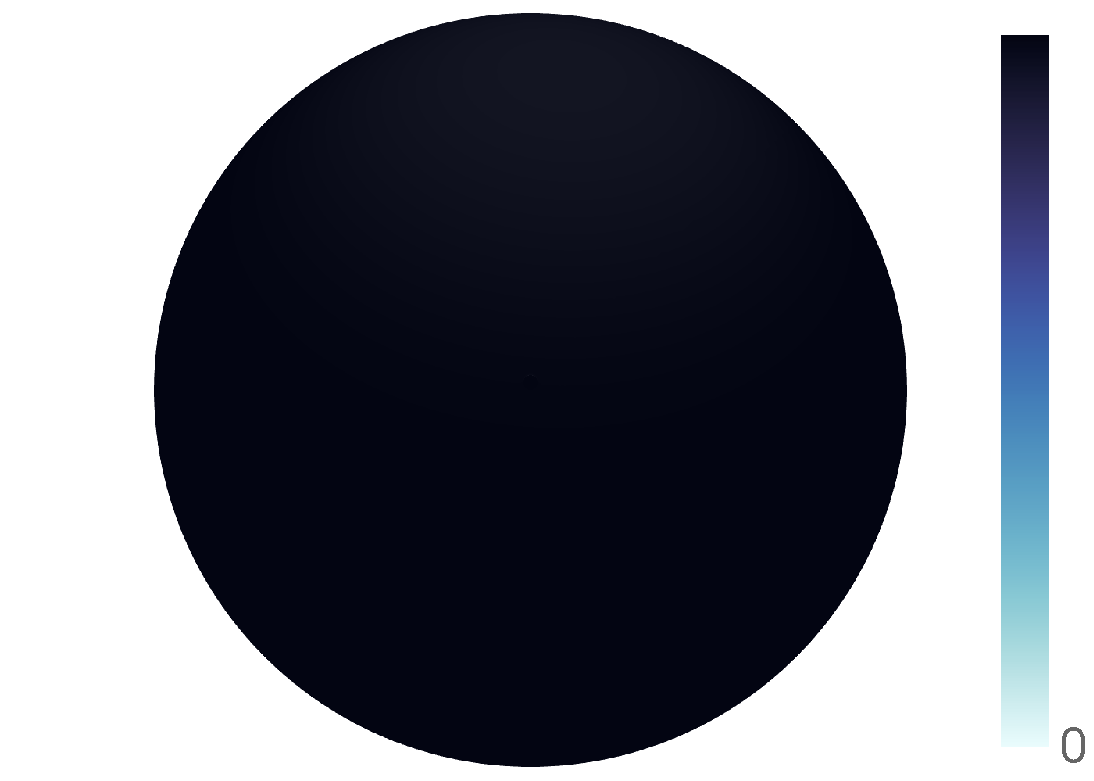
\includegraphics[trim={23 7 3 6},clip,width=.2\textwidth]{spherical_harmonic_0l_0m_L128_real_norm.pdf}}
	\newline
	\subfloat[\(\pixel{Y_{10}}\)]
	{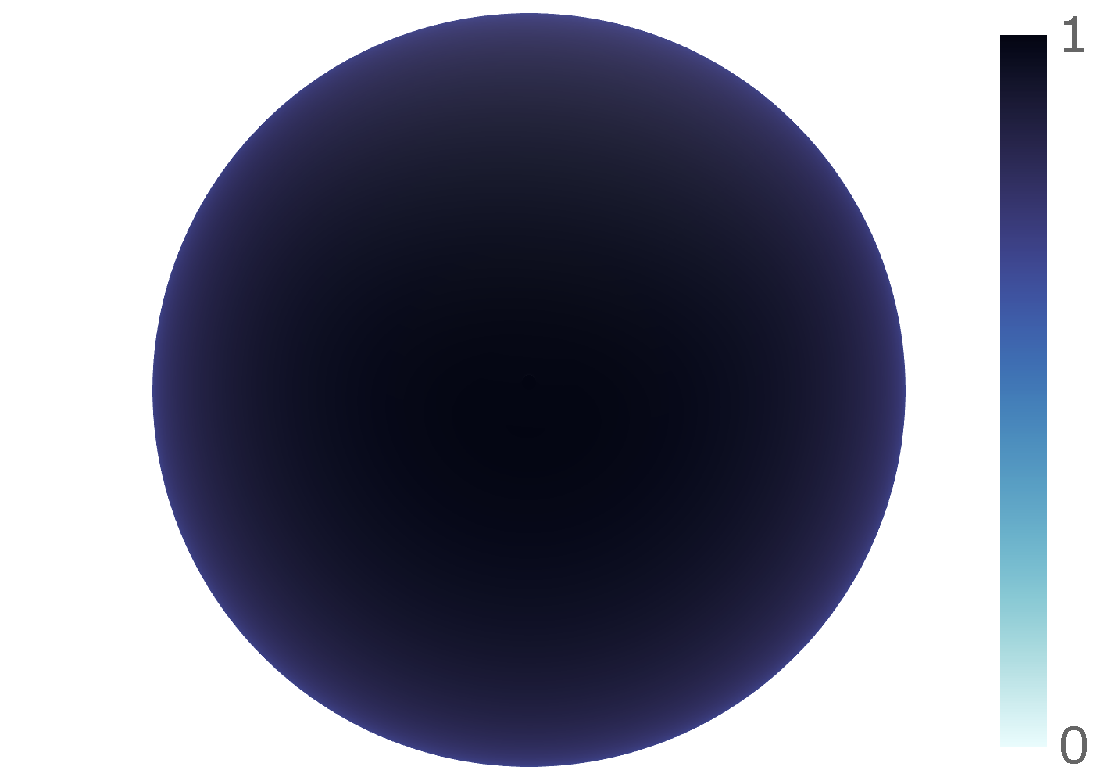
\includegraphics[trim={23 7 3 6},clip,width=.2\textwidth]{spherical_harmonic_1l_0m_L128_real_norm.pdf}}
	%
	\subfloat[\(\pixel{Y_{11}}\)]
	{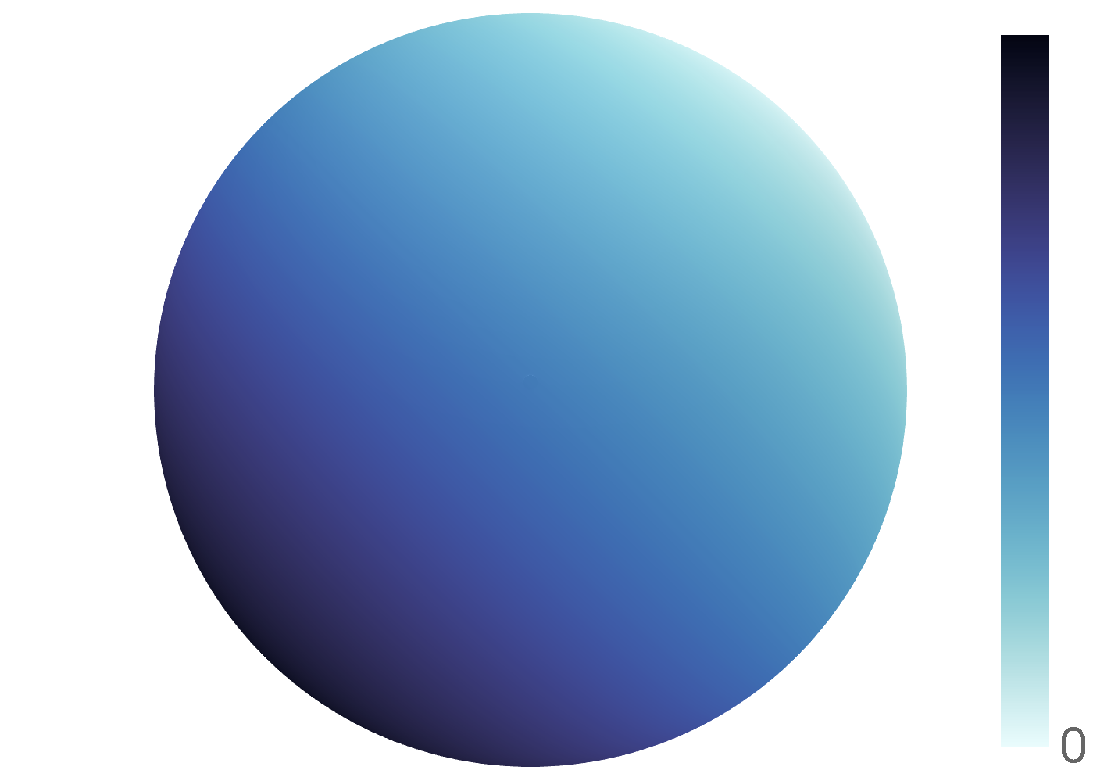
\includegraphics[trim={23 7 3 6},clip,width=.2\textwidth]{spherical_harmonic_1l_1m_L128_real_norm.pdf}}
	\newline
	\subfloat[\(\pixel{Y_{20}}\)]
	{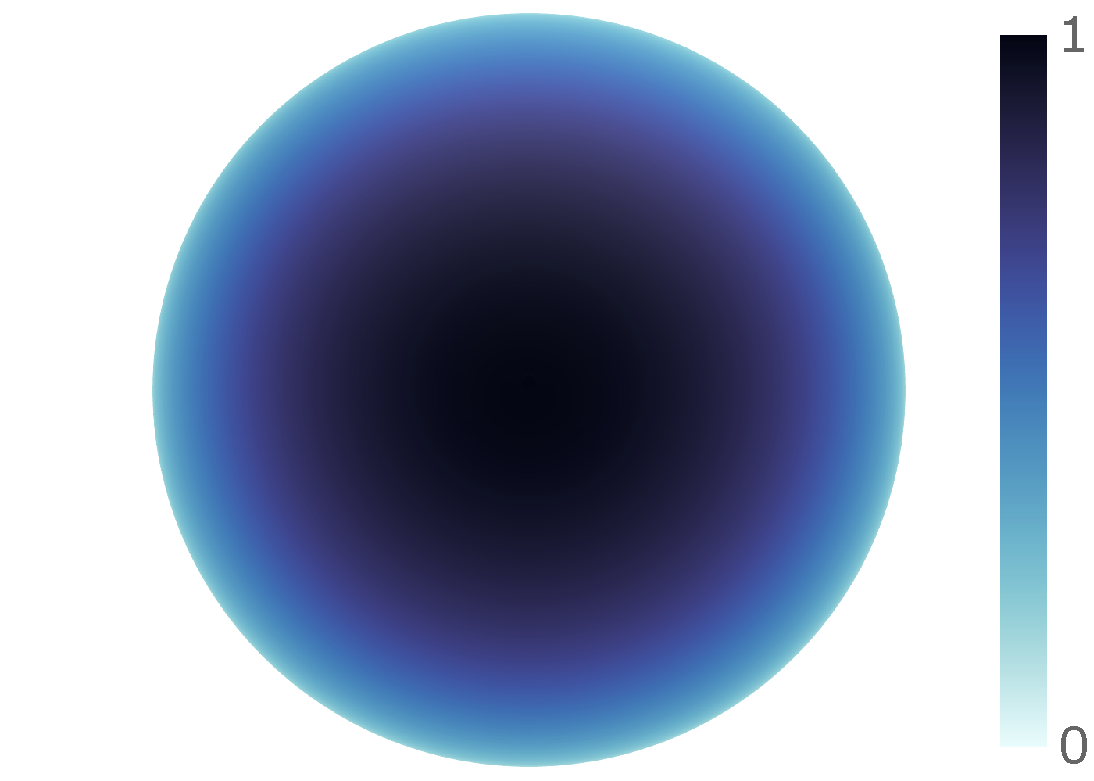
\includegraphics[trim={23 7 3 6},clip,width=.2\textwidth]{spherical_harmonic_2l_0m_L128_real_norm.pdf}}
	%
	\subfloat[\(\pixel{Y_{21}}\)]
	{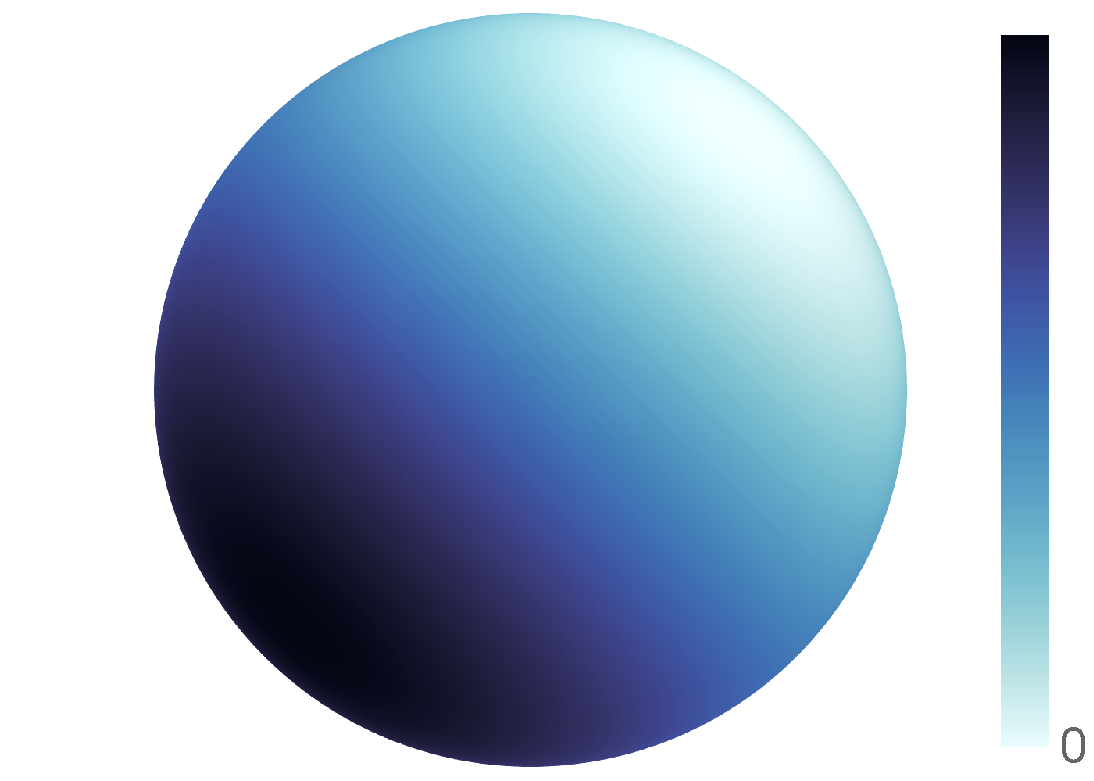
\includegraphics[trim={23 7 3 6},clip,width=.2\textwidth]{spherical_harmonic_2l_1m_L128_real_norm.pdf}}
	%
	\subfloat[\(\pixel{Y_{22}}\)]
	{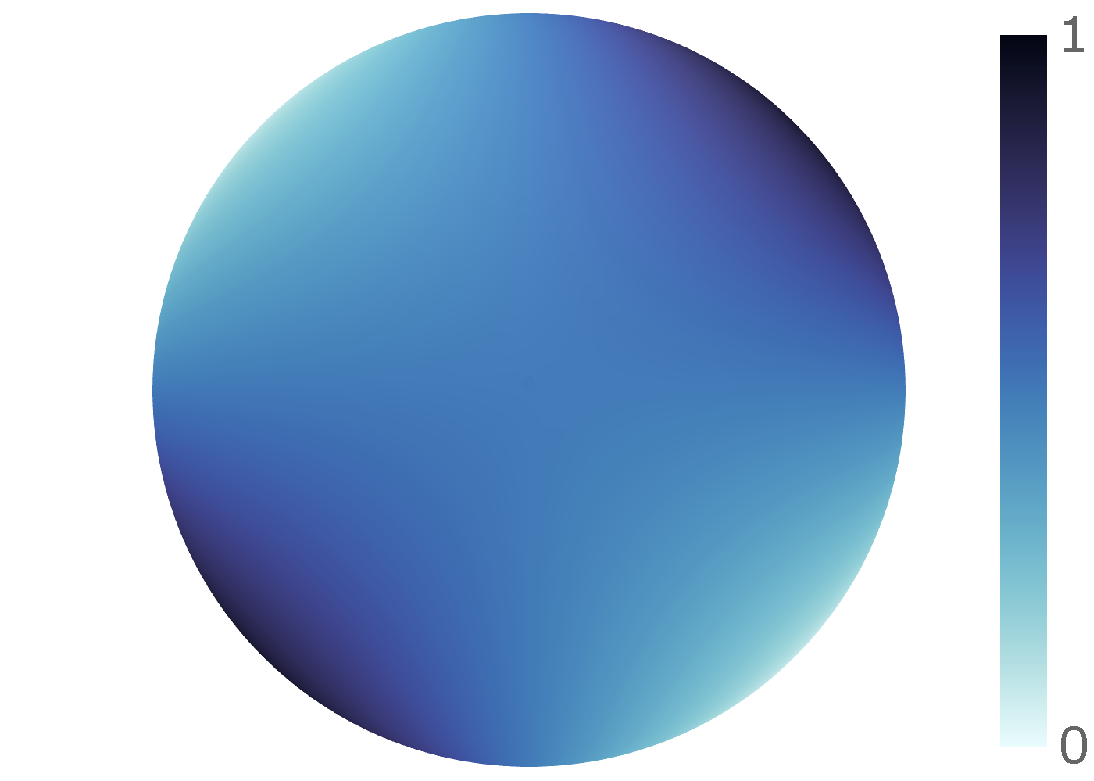
\includegraphics[trim={23 7 3 6},clip,width=.2\textwidth]{spherical_harmonic_2l_2m_L128_real_norm.pdf}}
	\newline
	\subfloat[\(\pixel{Y_{30}}\)]
	{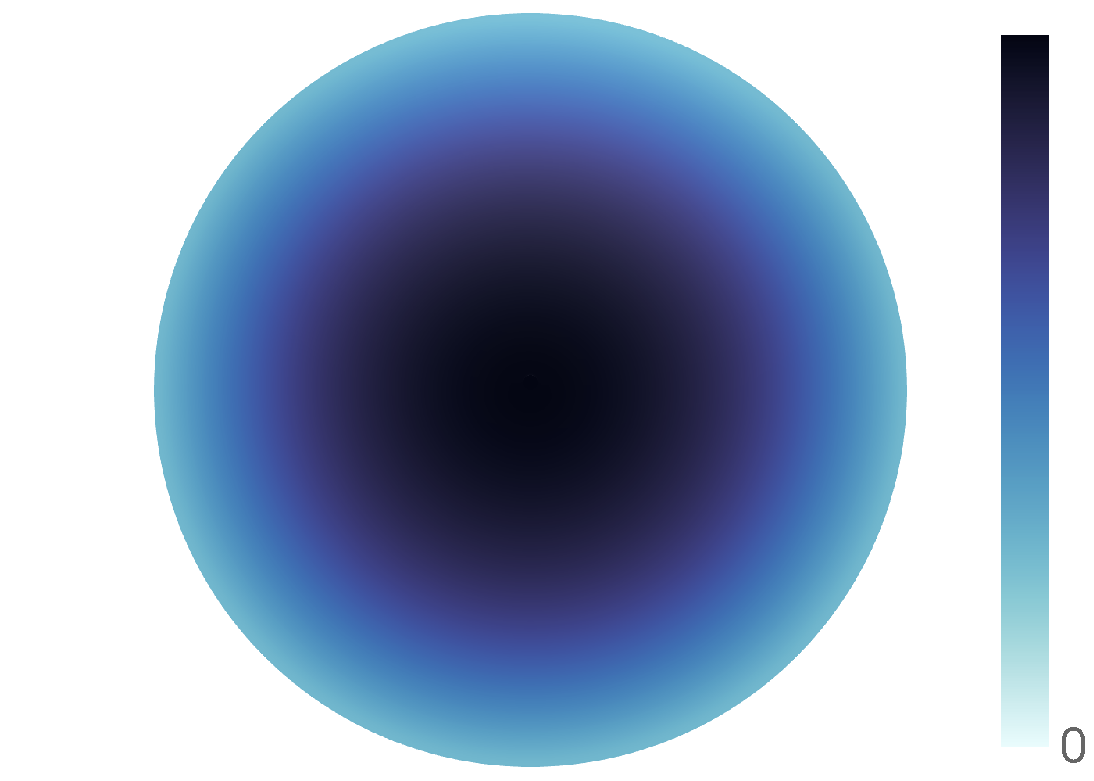
\includegraphics[trim={23 7 3 6},clip,width=.2\textwidth]{spherical_harmonic_3l_0m_L128_real_norm.pdf}}
	%
	\subfloat[\(\pixel{Y_{31}}\)]
	{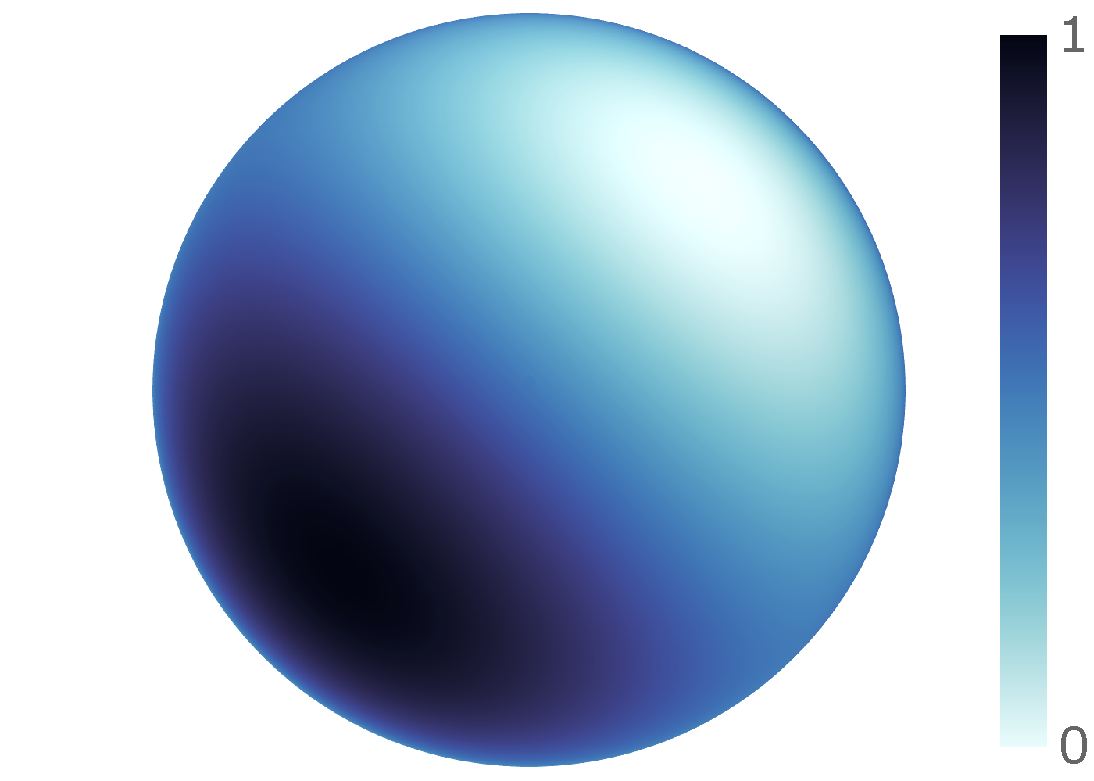
\includegraphics[trim={23 7 3 6},clip,width=.2\textwidth]{spherical_harmonic_3l_1m_L128_real_norm.pdf}}
	%
	\subfloat[\(\pixel{Y_{32}}\)]
	{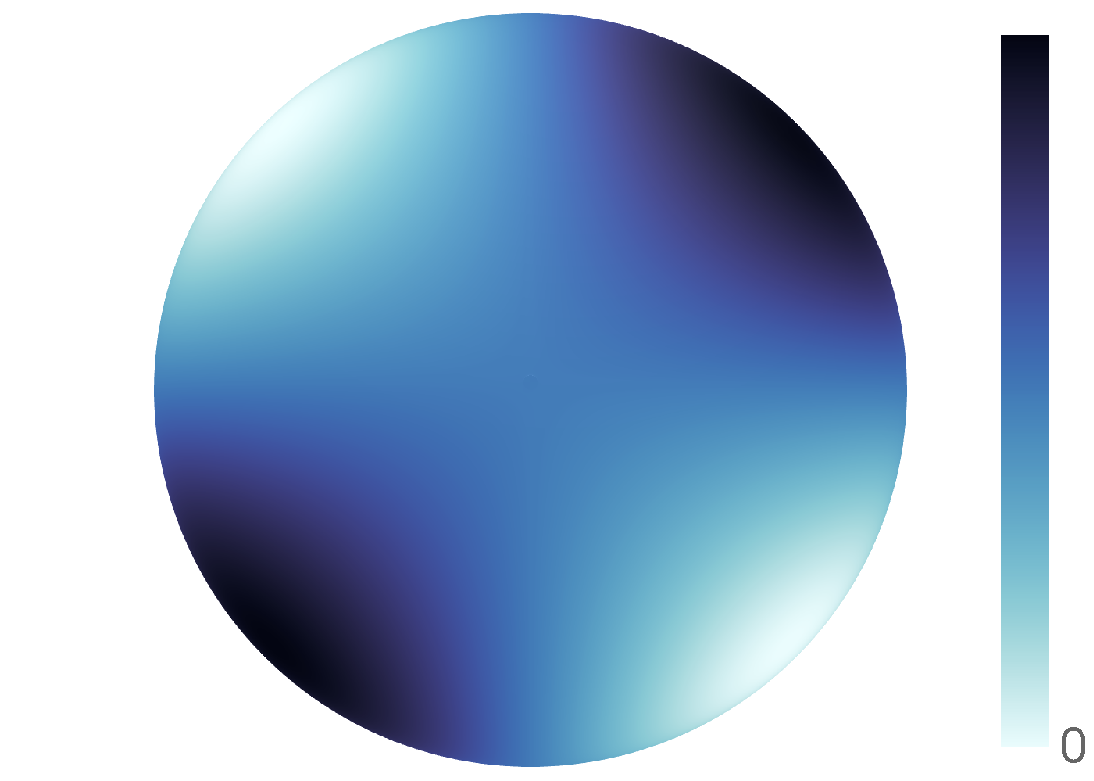
\includegraphics[trim={23 7 3 6},clip,width=.2\textwidth]{spherical_harmonic_3l_2m_L128_real_norm.pdf}}
	%
	\subfloat[\(\pixel{Y_{33}}\)]
	{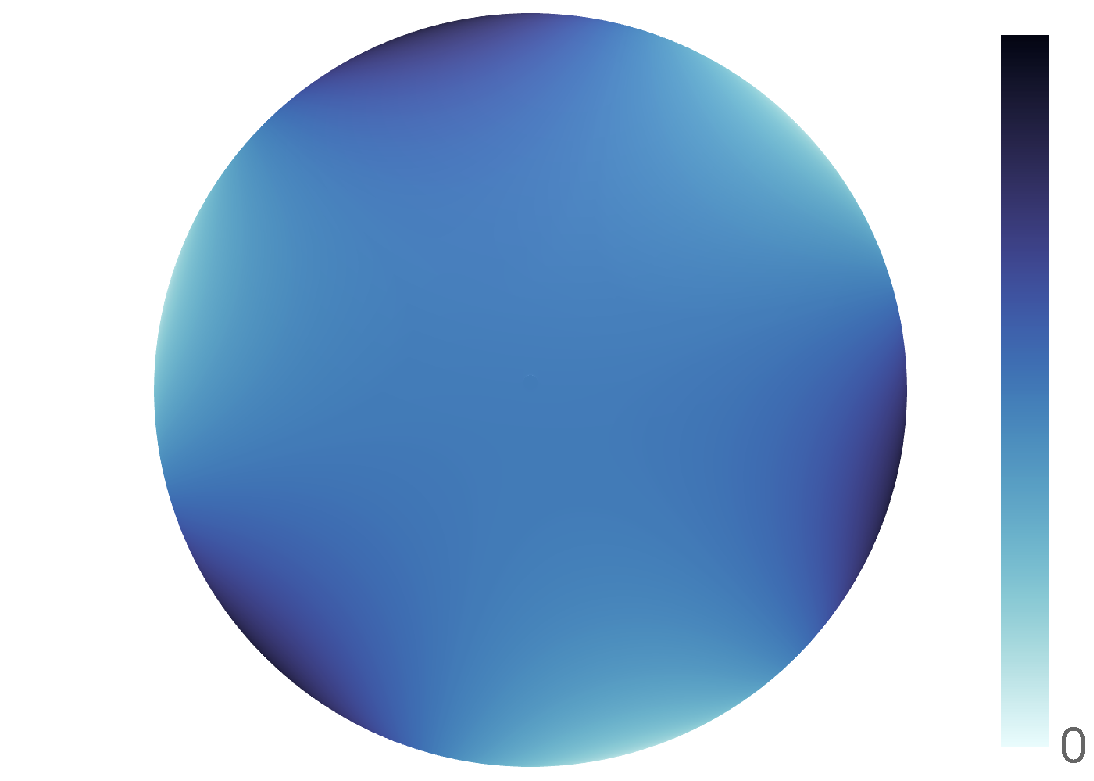
\includegraphics[trim={23 7 3 6},clip,width=.2\textwidth]{spherical_harmonic_3l_3m_L128_real_norm.pdf}}
	\newline
	\subfloat[\(\pixel{Y_{40}}\)]
	{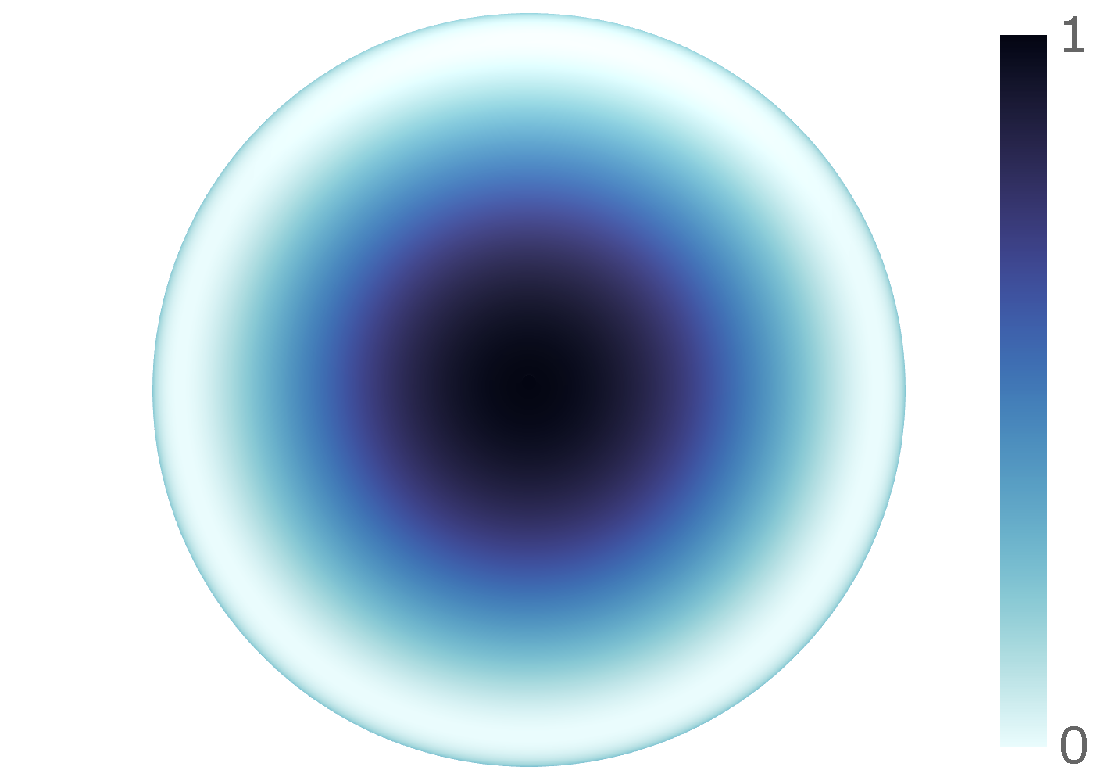
\includegraphics[trim={23 7 3 6},clip,width=.2\textwidth]{spherical_harmonic_4l_0m_L128_real_norm.pdf}}
	%
	\subfloat[\(\pixel{Y_{41}}\)]
	{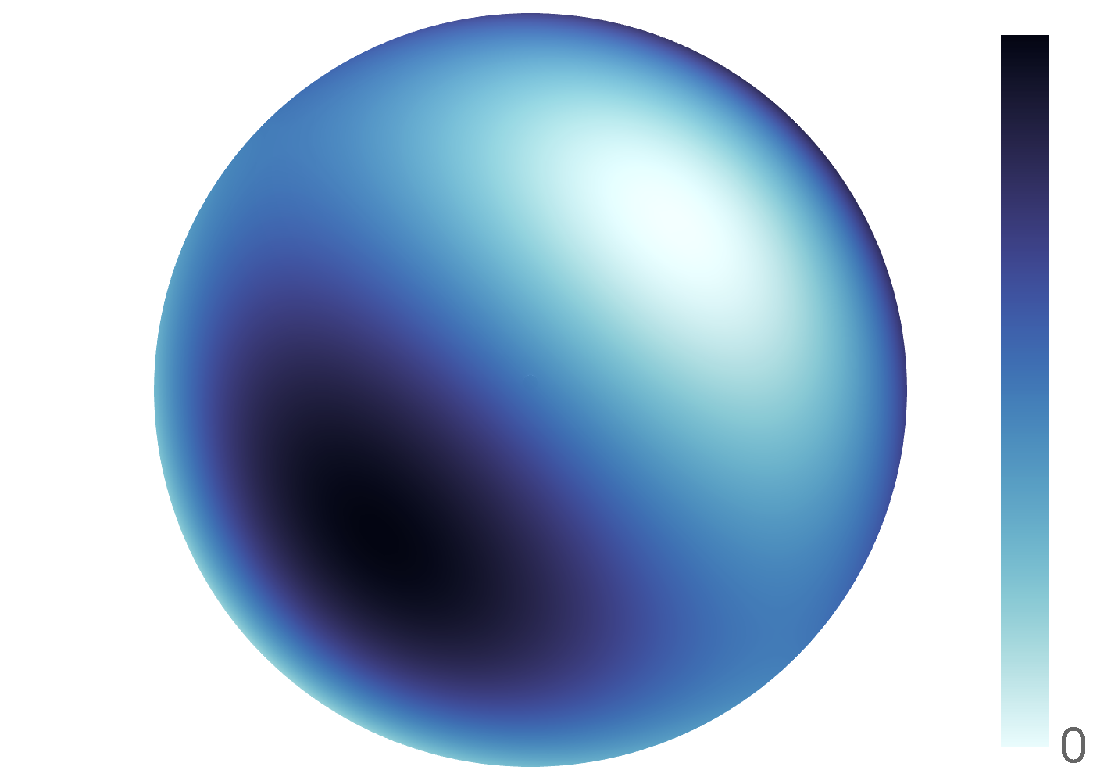
\includegraphics[trim={23 7 3 6},clip,width=.2\textwidth]{spherical_harmonic_4l_1m_L128_real_norm.pdf}}
	%
	\subfloat[\(\pixel{Y_{42}}\)]
	{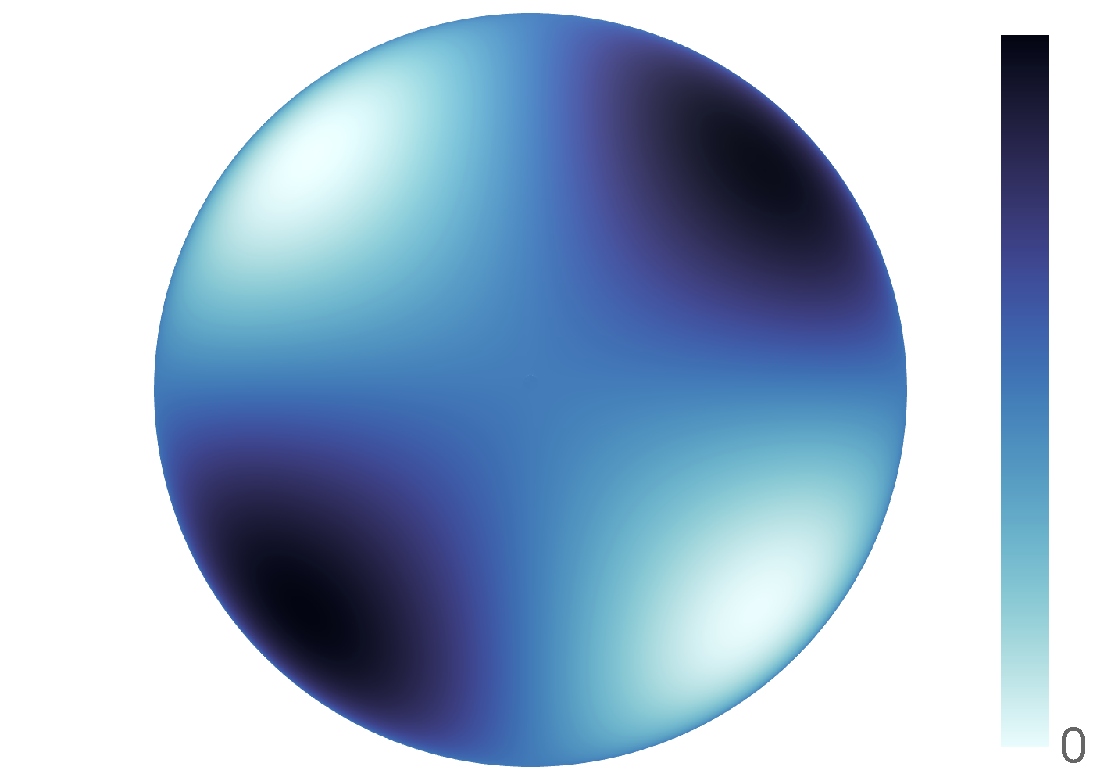
\includegraphics[trim={23 7 3 6},clip,width=.2\textwidth]{spherical_harmonic_4l_2m_L128_real_norm.pdf}}
	%
	\subfloat[\(\pixel{Y_{43}}\)]
	{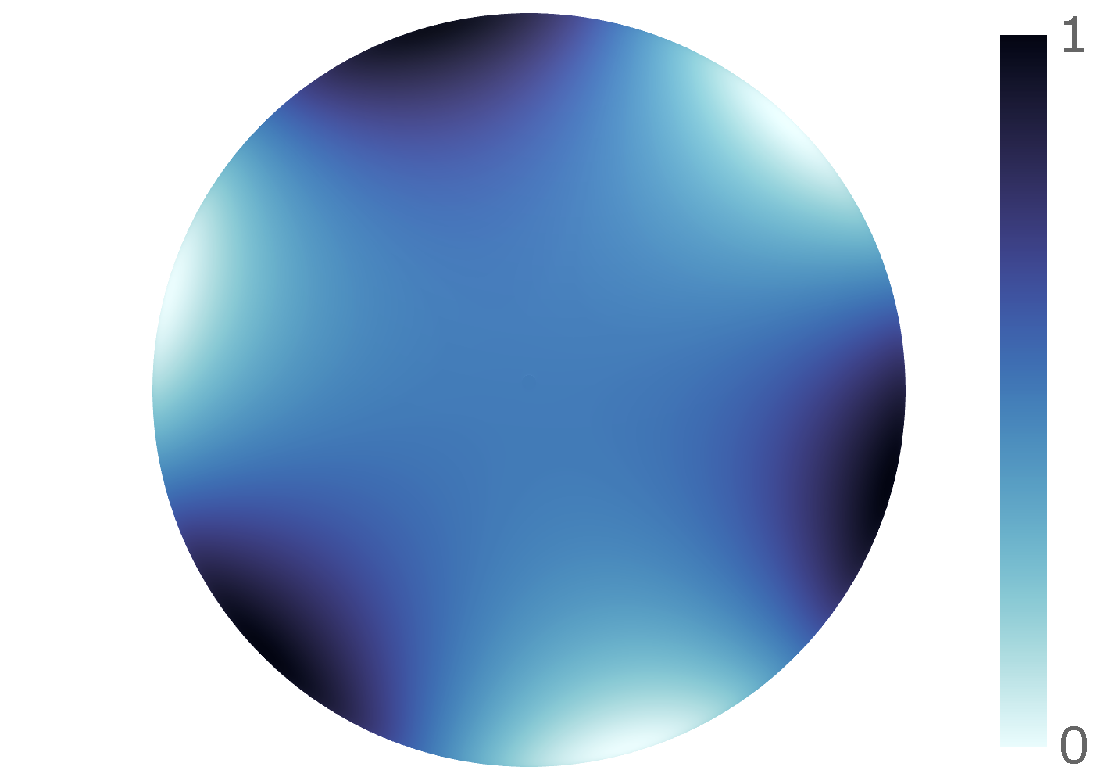
\includegraphics[trim={23 7 3 6},clip,width=.2\textwidth]{spherical_harmonic_4l_3m_L128_real_norm.pdf}}
	%
	\subfloat[\(\pixel{Y_{44}}\)]
	{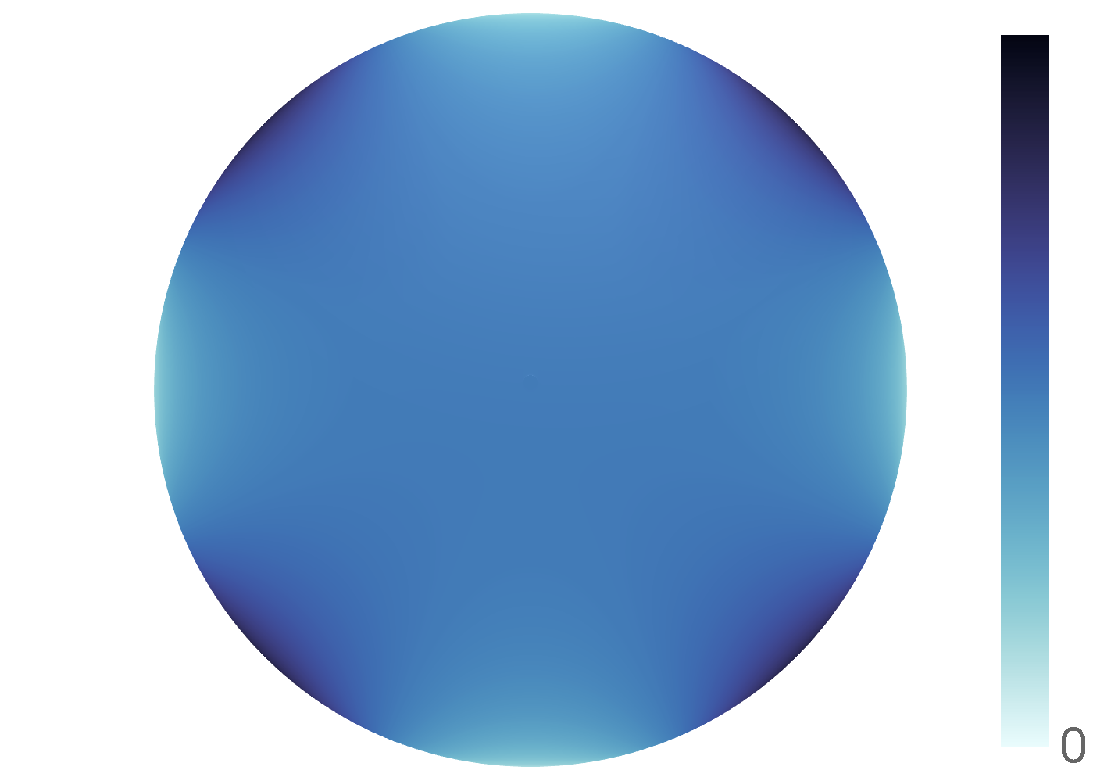
\includegraphics[trim={23 7 3 6},clip,width=.2\textwidth]{spherical_harmonic_4l_4m_L128_real_norm.pdf}}
	\caption[
		The spherical harmonics for \(\ell=0,\ldots,4\)
	]{
		The real part of the spherical harmonics \(\pixel{\harmonic{Y}}\) for \(\ell=0,\ldots,4\) (top-to-bottom) and \(m=0,\ldots,\ell{}\) (left-to-right).
		The negative order harmonics \(\pixel{Y_{\ell(-m)}}\) have not been included as they are simply rotated with respect to the positive order harmonics by \(\SI{90}{\degree}/m\).
	}\label{fig:chapter2_spherical_harmonics}
\end{figure}


\subsection{Rotations on the Sphere}

Rotations of functions defined on the sphere form an integral part of analysis on the sphere.
The Euler angles \(\rho=(\alpha,\beta,\gamma) \in \rotationGroup{}\) may parametrise three-dimensional rotations, where \(\alpha \in \interval[open right]{0}{2\pi}\), \(\beta \in \interval{0}{\pi}\), and \(\gamma \in \interval[open right]{0}{2\pi}\).
The sequence of rotations:
%
\begin{enumerate}[(i),nosep,left=\parindent]
	\item \({\gamma}\) rotation about the \(z\)-axis;
	\item \({\beta}\) rotation about the \(y\)-axis; and
	\item \({\alpha}\) rotation about the \(z\)-axis;
\end{enumerate}
%
define the rotation operator \(\rotation{\rho}\).
A function \(\pixel{f} \in \hilbert{\twoSphere}\) rotated on the sphere is defined by
%
\begin{equation}
	\pixel{(\rotation{\rho}f)}
	%
	= f(\rotationMatrix^{-1} \omega),
\end{equation}
%
where \(\rotationMatrix{}\) is the three-dimensional rotation matrix corresponding to \(\rotation{\rho}\).
A rotation of a spherical harmonic function may be represented by
%
\begin{equation}\label{eq:chapter2_wigner_ylm}
	\rotation{\rho} \pixel{\harmonic{Y}}
	%
	= \sum\limits_{n=-\ell}^{\ell} \wigner{\ell}{n}{m}(\rho) \pixel{Y_{\ell n}},
\end{equation}
%
where \(\wigner{\ell}{n}{m}(\rho)\) are the \emph{Wigner D matrices}~\cite{Brink1993,Ritchie1999}.
The Wigner D matrices form the \(2\ell+1\)-dimensional representation of the rotation group \(\rotationGroup{}\) for a given \(\ell{}\) and are given by
%
\begin{equation}
	\wigner{\ell}{n}{m}(\rho)
	%
	= \exp(-i n\alpha) \reducedWigner{\ell}{n}{m}(\beta) \exp(-i m\gamma),
\end{equation}
%
where \(\reducedWigner{\ell}{n}{m}(\beta)\) are the \emph{reduced d matrices} which are real in this phase convention and satisfy many symmetry relations.
By the \emph{Peter-Weyl} theorem, the matrix elements \(\wigner{\ell}{n}{m}(\rho)\) form an orthonormal basis on \(\hilbert{\rotationGroup}\), \ie{}
%
\begin{equation}
	\integrateRotation{\rho} \wigner{\ell}{n}{m}(\rho) \wigner[\ast]{\ell'}{n'}{m'}(\rho)
	%
	= \frac{8\pi^{2}}{2\ell+1} \delta_{\ell\ell'} \delta_{nn'} \delta_{mm'},
\end{equation}
%
where \(\rotationVolume = \sin{\beta}\dd{\alpha}\dd{\beta}\dd{\gamma}\) is the usual invariant measure on \(\rotationGroup{}\).
%
It follows that the harmonic coefficients of a rotated function read
%
\begin{equation}
	\harmonic{(\rotation{\rho}f)}
	%
	= \sum\limits_{n=-\ell}^{\ell} \wigner{\ell}{m}{n}(\rho) f_{\ell n}.
\end{equation}
%
Note the order of the indices on \(\wigner{\ell}{m}{n}(\rho)\) here compared to \cref{eq:chapter2_wigner_ylm}.
The spherical harmonics are related to the axisymmetric rotation matrices by
%
\begin{equation}
	\wigner[\ast]{\ell}{m}{0}(\phi,\theta,0)
	%
	= \sqrt{\inverseFactor} \pixel{\harmonic{Y}}.
\end{equation}

\section{Wavelets}\label{sec:chapter2_wavelets}

\subsection{Euclidean}

\subsection{Sphere}

\begin{figure}[htpb]
	\centering\capstart{}
	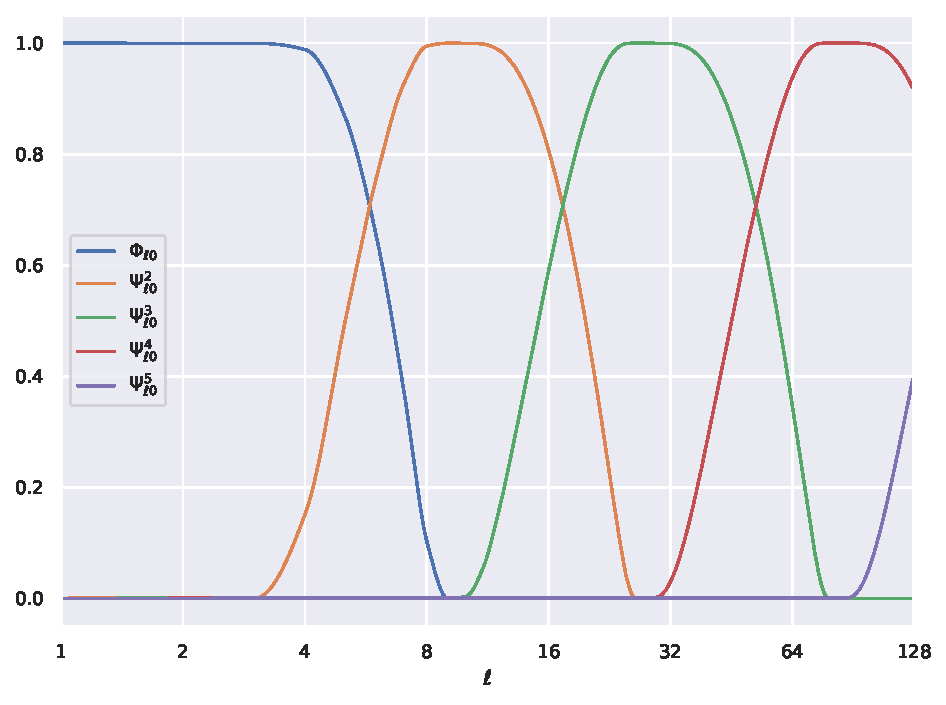
\includegraphics[width=\textwidth]{axisymmetric_tiling_L128.pdf}
	\caption[
	]{
	}\label{fig:chapter2_tiling}
\end{figure}


\begin{figure}[htpb]
	\centering\capstart{}
	\subfloat[\(\pixel{\Phi}\)]
	{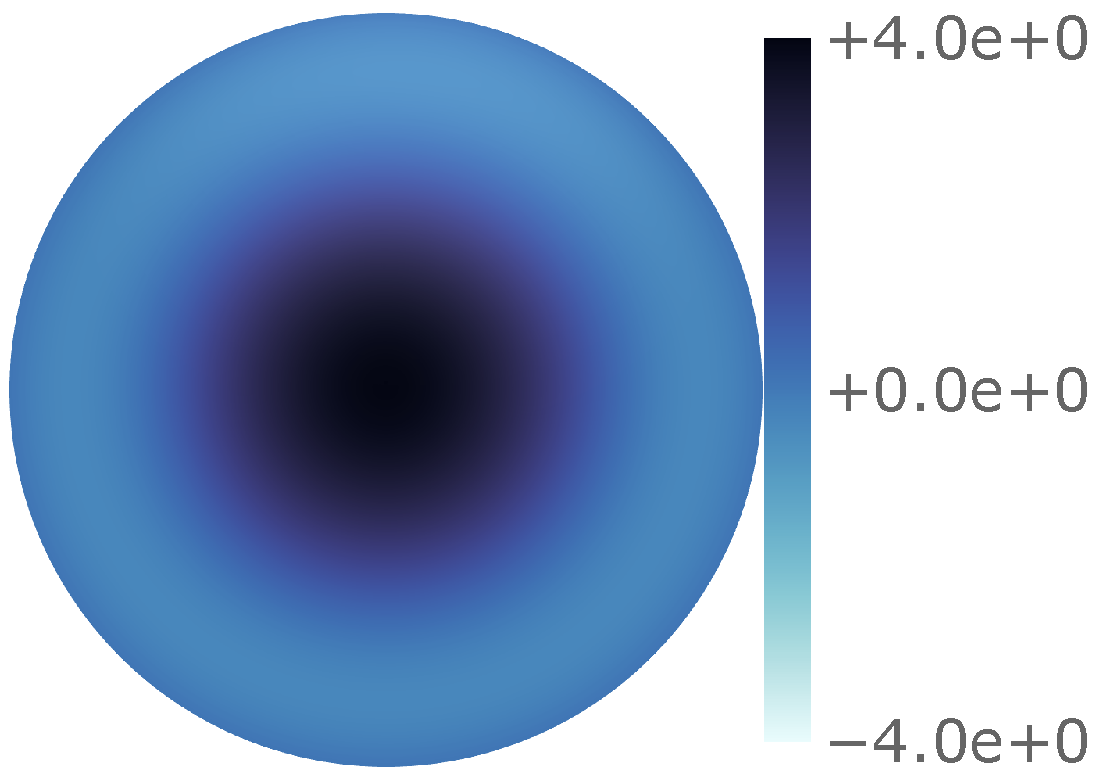
\includegraphics[trim={4 7 3 6},clip,width=.33\textwidth]{axisymmetric_wavelets_3B_2jmin_scaling_L128_res512_real.pdf}}
	\hfill
	\subfloat[\(\pixel{\Psi^{2j}}\)]
	{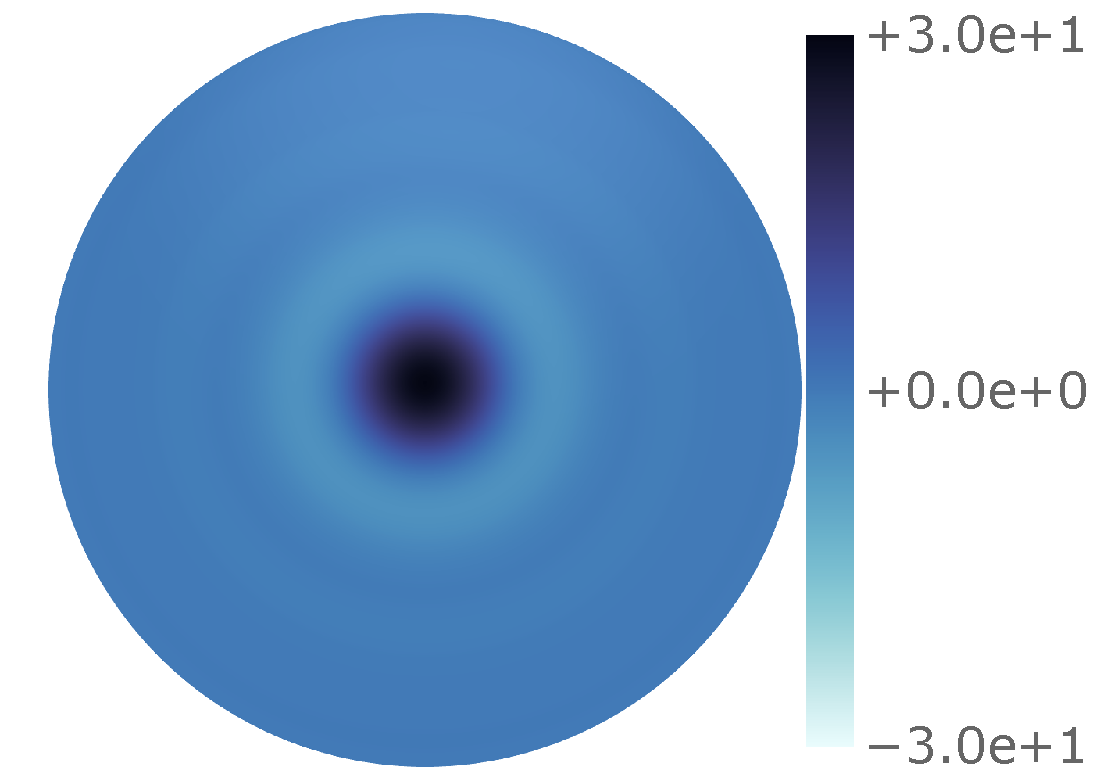
\includegraphics[trim={4 7 3 6},clip,width=.33\textwidth]{axisymmetric_wavelets_3B_2jmin_2j_L128_res512_real.pdf}}
	\hfill
	\subfloat[\(\pixel{\Psi^{3j}}\)]
	{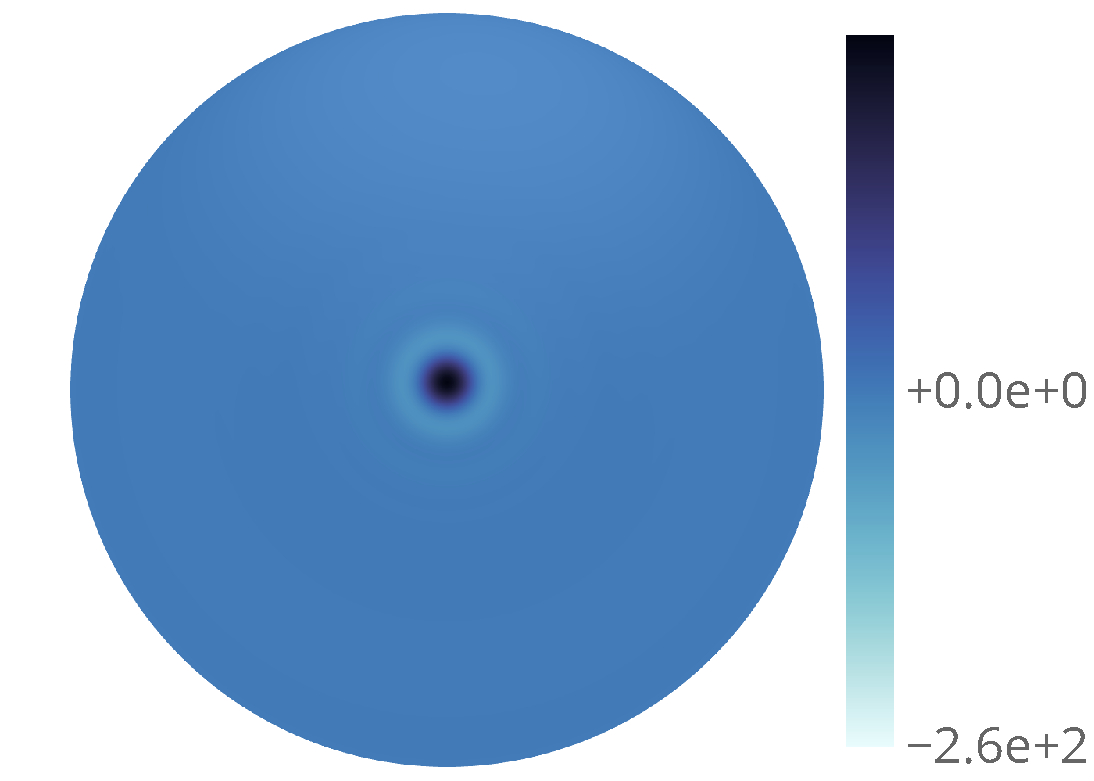
\includegraphics[trim={4 7 3 6},clip,width=.33\textwidth]{axisymmetric_wavelets_3B_2jmin_3j_L128_res512_real.pdf}}
	\newline
	\subfloat[\(\pixel{\Psi^{4j}}\)]
	{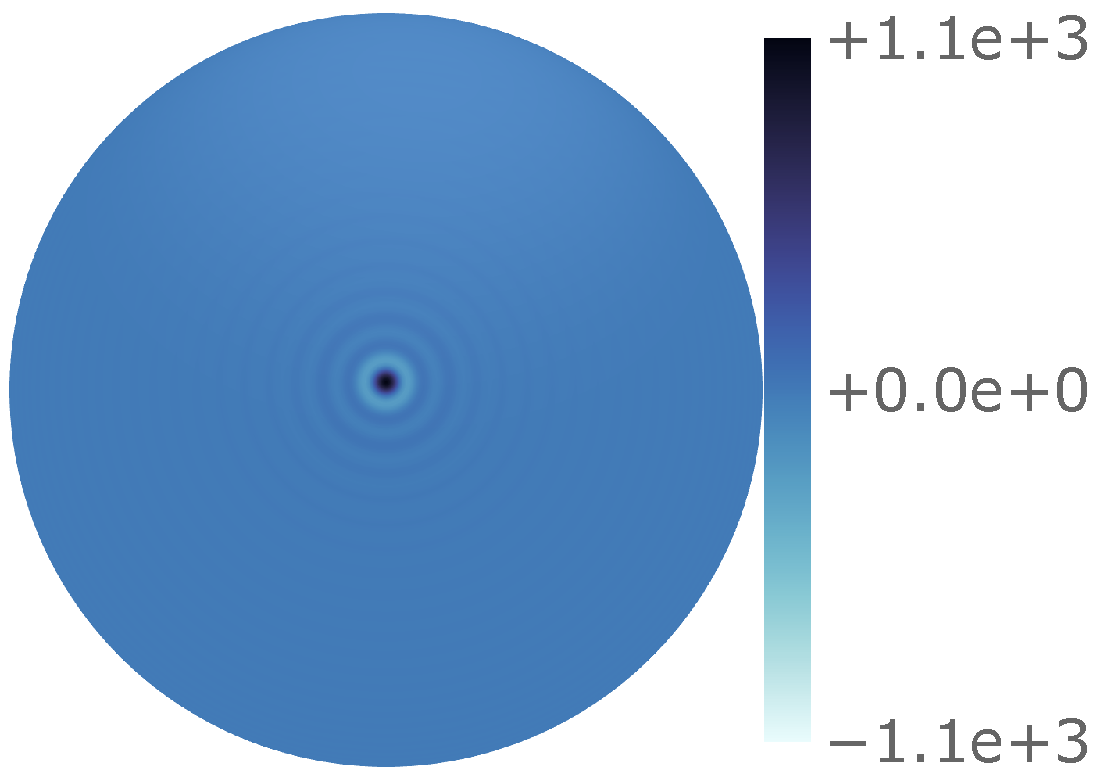
\includegraphics[trim={4 7 3 6},clip,width=.33\textwidth]{axisymmetric_wavelets_3B_2jmin_4j_L128_res512_real.pdf}}
	%
	\subfloat[\(\pixel{\Psi^{5j}}\)]
	{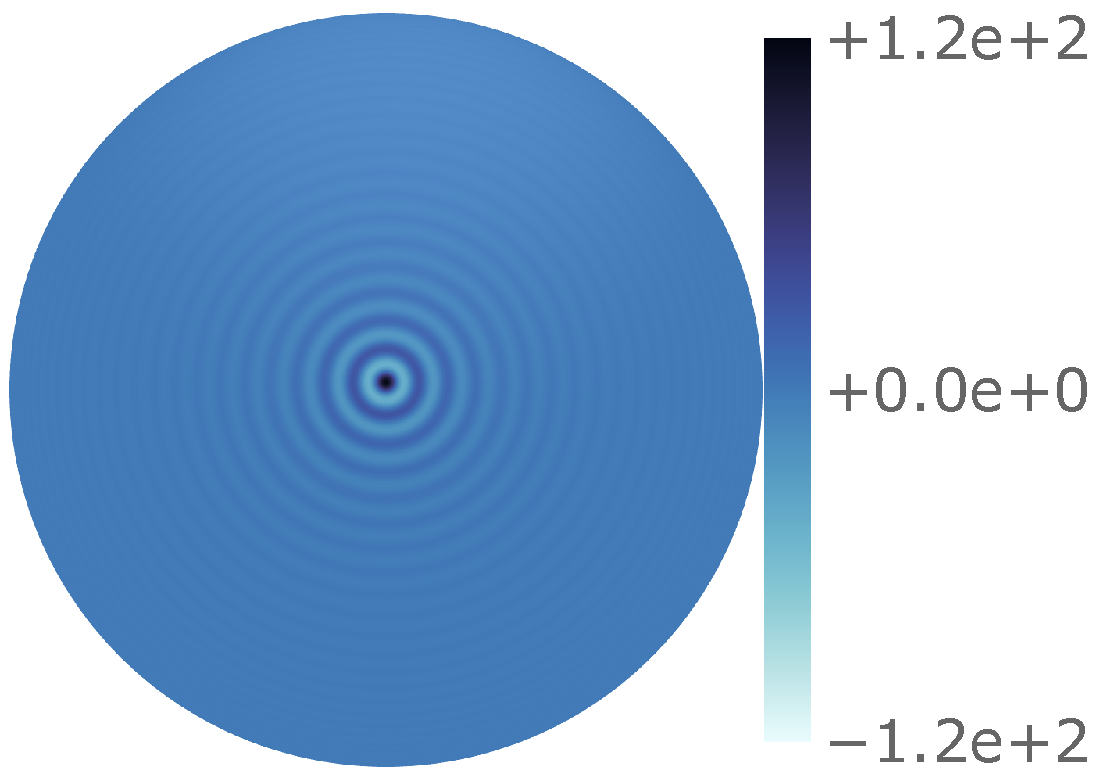
\includegraphics[trim={4 7 3 6},clip,width=.33\textwidth]{axisymmetric_wavelets_3B_2jmin_5j_L128_res512_real.pdf}}
	\caption[
		Some axisymmetric scale-discretised wavelets on the sphere
	]{
		The scaling function and the wavelets for scales \(j \in \set{2, 3, 4, 5}\) of the axisymmetric scale-discretised wavelets on the sphere centred on the north pole shown left-to-right, top-to-bottom.
		They are constructed through a tiling of the harmonic line with parameters \(\lambda=3\), \(J_{0}=2\), and bandlimit \(L=128\) (\cf{} \cref{fig:chapter2_tiling}).
	}\label{fig:chapter2_axisymmetric_wavelets}
\end{figure}


\section{Slepian Concentration Problem}\label{sec:chapter2_slepian_concentration_problem}

In the 1960s, Slepian, Landau and Pollak solved the fundamental problem of optimally concentrating a signal simultaneously in time and frequency~\cite{Landau1961,Landau1962,Slepian1983,Slepian1961}.
The resulting orthogonal family of functions, and their discrete and multidimensional counterparts~\cite{Bronez1988,Hanssen1997,Liu1992,Slepian1964,Slepian1978}, form the basis of a range of spectral analyses (\eg{}~\cite{Thomson1982,Thomson1990}).
\cref{sec:chapter2_slepian_euclidean} follows with a brief review of the initial time-frequency concentration problem, this is then proceeded with the extension to the spherical domain in \cref{sec:chapter2_slepian_sphere}.

\subsection{Euclidean: Time-Frequency Domain}\label{sec:chapter2_slepian_euclidean}

Before considering the Slepian spatial-spectral concentration problem in the spherical domain, first consider the one-dimensional, continuous-continuous, time-frequency concentration problem.
Here, a normalisation convention is adopted such that a real-valued time-domain single \(f(t)\) and its Fourier transform \(F(\varpi)\) are related by
%
\begin{equation}
	f(t)
	%
	= \frac{1}{2\pi} \int\limits_{-\infty}^{\infty} \dd{\varpi} F(\varpi) \exp(i\varpi t)
\end{equation}
%
and
%
\begin{equation}
	F(\varpi)
	%
	= \int\limits_{-\infty}^{\infty} \dd{\varpi} f(t) \exp(-i\varpi t),
\end{equation}
%
where \(t\) and \(\varpi{}\) denote the time and angular frequency respectively.
Slepian and Pollak~\cite{Slepian1961} considered the problem of optimally concentrating a strictly bandlimited signal \(f(t)\), with a spectrum \(F(\varpi)\) which disappears into a time interval \(\abs{t} \leq T\) for frequencies \(\abs{\varpi} > W\).
Through the \emph{Paley-Wiener} theorem, no bandlimited signal \(g(t)\) can be exactly concentrated within a finite interval~\cite{Daubechies1992,Mallat2008}.
To find the optimally concentrated signal, one must maximise the following ratio:
%
\begin{equation}\label{eq:chapter2_frequency_ratio}
	\mu
	%
	= \frac{\displaystyle\int\limits_{-T}^{T} \dd{t} \abs{g(t)}^{2}}
	%
	{\displaystyle\int\limits_{-\infty}^{\infty} \dd{t} \abs{g(t)}^{2}},
\end{equation}
%
although other criteria have been considered~\cite{Freeden1997,Riedel1995}.
Bandlimited signals \(g(t)\) which satisfy \cref{eq:chapter2_frequency_ratio}, have spectra \(G(\varpi)\) which satisfy the convolutional integral eigenproblem in the frequency-domain
%
\begin{equation}\label{eq:chapter2_frequency_eigenproblem}
	\int\limits_{-W}^{W} \dd{\varpi'} \frac{\sin{T(\varpi-\varpi')}}{\pi(\varpi-\varpi')} G(\varpi')
	%
	= \mu G(\varpi),
\end{equation}
%
where \(\abs{\varpi} \leq W\).

Slepian \etal{} also considered the similar case of concentrating the spectrum \(H(\varpi)\) of a strictly timelimited function \(h(t)\), which disappears into a spectral interval \(\abs{\varpi} \leq W\) for times \(\abs{t} > T\).
The ratio to maximise here is
%
\begin{equation}\label{eq:chapter2_time_ratio}
	\mu
	%
	= \frac{\displaystyle\int\limits_{-W}^{W} \dd{\varpi} \abs{H(\varpi)}^{2}}
	%
	{\displaystyle\int\limits_{-\infty}^{\infty} \dd{\varpi} \abs{H(\varpi)}^{2}},
\end{equation}
%
which results in the time-domain eigenproblem
%
\begin{equation}\label{eq:chapter2_time_eigenproblem}
	\int\limits_{-T}^{T} \dd{t'} \frac{\sin{W(t-t')}}{\pi(t-t')} h(t')
	%
	= \mu h(t),
\end{equation}
%
where \(\abs{t} < T\).
In either case, the eigenvalues (which represent effective concentration) satisfy
%
\begin{equation}
	1 > \mu_{1} \geq \mu_{2} \geq \ldots > 0, % chktex 11
\end{equation}
%
with associated eigenfunctions, \eg{}
%
\begin{equation}
	g_{1}(t),\ g_{2}(t),\ \ldots
\end{equation}
%
which exist in the interval \(\abs{t} \leq T\).
Through a change of variables, the ratios \cref{eq:chapter2_frequency_ratio,eq:chapter2_time_ratio} may be transformed into one dimensionless eigenproblem:
%
\begin{equation}
	\int\limits_{-1}^{1} \dd{x'} \frac{\sin{TW(x-x')}}{\pi(x-x')} \psi(x')
	%
	= \mu \psi(x),
\end{equation}
%
where \(\abs{x} \leq 1\).
Hence, the eigenvalues and scaled eigenfunctions only depend on the time-bandwith product \(TW\).
Consider the sum of the eigenvalues
%
\begin{equation}
	N
	%
	= \sum\limits_{p=1}^{\infty} \mu_{p}
	%
	= \frac{2TW}{\pi}.
\end{equation}
%
The so-called Shannon number~\cite{Percival1993} \(N\) introduced here is a good estimate of the number of significant eigenvalues, which arises due to the characteristic shape of the eigenvalue spectrum~\cite{Landau1965,Slepian1965} (see \cref{fig:chapter2_polar_cap_eigenvalues}).
Equivalently, this can be viewed as the number of signals \(f(t)\) which can be well-concentrated both into a finite time interval \(\abs{t} \leq T\) and a finite frequency interval \(\abs{\varpi} \leq W\).
Many of the results discussed above have analogues in the spatial-spectral concentration problem on the sphere, which is elaborated in \cref{sec:chapter2_slepian_sphere}.

\subsection{Sphere: Spatial-Spectral Domain}\label{sec:chapter2_slepian_sphere}

The two sub-spaces of interest of all square-integrable functions on the sphere \(\twoSphere{}\) are: \(\spaceSpacelimit{}\) the space of all spacelimited functions strictly contained within a region \(R\), and \(\spaceBandlimit{}\) the space of all bandlimited functions with no power above the bandlimit \(L\).
Akin to the Euclidean setting, no function can be strictly spacelimited as well as strictly bandlimited, \ie{} no \(\pixel{f}\) can be in both sub-spaces \(\spaceSpacelimit{}\) and \(\spaceBandlimit{}\) at the same time.
Thus, one may find either: the spacelimited functions \(\pixel{h} \in \spaceSpacelimit{}\) whose spectrum is optimally concentrated within the interval \(0 \leq \ell < L\), or the bandlimited functions \(\pixel{g} \in \spaceBandlimit{}\) which are optimally concentrated within a region \(R\).

\subsubsection{Spectral Concentration of a Spacelimited Function}

To maximise the concentration of a spacelimited function \(\pixel{h} \in \spaceSpacelimit{}\) within an interval \(0 \leq \ell < L\) one must maximise the ratio:
%
\begin{equation}\label{eq:chapter2_spacelimited_ratio}
	\mu
	%
	= \frac{\displaystyle\sum\limits_{\ell=0}^{L-1} \sum\limits_{m=-\ell}^{\ell} \abs{\harmonic{h}}^{2}}
	%
	{\displaystyle\sum\limits_{\ell=0}^{\infty} \sum\limits_{m=-\ell}^{\ell} \abs{\harmonic{h}}^{2}},
\end{equation}
%
which is analogous to the one-dimensional problem \cref{eq:chapter2_time_ratio}.
By substituting the expansion of the spherical harmonic coefficients
%
\begin{equation}
	\harmonic{h}
	%
	= \integrateRegion{\sphereVolume} \pixel{h} \pixel{\conj{\harmonic{Y}}},
\end{equation}
%
and swapping the order of summation and integration, the variational problem \cref{eq:chapter2_spacelimited_ratio} becomes
%
\begin{equation}
	\mu
	%
	= \frac{\integrateRegion{\sphereVolume[']} \pixel[']{h} \integrateRegion{\sphereVolume} \pixel{\delta_{\omega'}} \pixel{\conj{h}}}
	%
	{\integrateRegion{\sphereVolume} \abs{\pixel{h}}^{2}},
\end{equation}
%
where
%
\begin{equation}
	\pixel{\delta_{\omega'}}
	%
	= \sum\limits_{\ell=0}^{L-1} \sum\limits_{m=-\ell}^{\ell} \pixel[']{\conj{\harmonic{Y}}} \pixel{\harmonic{Y}}
\end{equation}
%
is the bandlimited Dirac delta function.
The maximally spacelimited functions \(\pixel{h} \in \spaceSpacelimit{}\) are therefore the solutions to the integral equation
%
\begin{equation}
	\integrateRegion{\sphereVolume} \pixel{\delta_{\omega'}} \pixel{\conj{h}}
	%
	= \mu \pixel[']{\conj{h}},
\end{equation}
%
which is the spherical analogue of the one-dimensional time-domain eigenproblem \cref{eq:chapter2_time_eigenproblem}.

\subsubsection{Spatial Concentration of a Bandlimited Function}

Conversely, to find the maximally concentrated bandlimited functions \(\pixel{g} \in \spaceBandlimit{}\) within a region \(R\) one must maximise the ratio:
%
\begin{equation}\label{eq:chapter2_bandlimited_ratio}
	\mu
	%
	= \frac{\integrateRegion{\sphereVolume} \abs{\pixel{g}}^{2}}
	%
	{\integrateSphere{\omega} \abs{\pixel{g}}^{2}},
\end{equation}
%
which is, as before, analogous to the one-dimensional problem \cref{eq:chapter2_frequency_ratio}.
Expanding in harmonic space, and swapping the order of summation and integration, \cref{eq:chapter2_bandlimited_ratio} becomes
%
\begin{equation}
	\mu
	%
	= \frac{\displaystyle\sum\limits_{\ell=0}^{L-1} \sum\limits_{m=-\ell}^{\ell} \harmonic{g}
		%
		\sum\limits_{\ell'=0}^{L-1} \sum\limits_{m'=-\ell'}^{\ell'} \Dmatrix \conj{\harmonic[']{g}}}
	%
	{\displaystyle\sum\limits_{\ell=0}^{L-1} \sum\limits_{m=-\ell}^{\ell} \abs{\harmonic{g}}^{2}},
\end{equation}
%
where
%
\begin{equation}
	\Dmatrix
	%
	= \integrateRegion{\sphereVolume} \pixel{\harmonic{Y}} \pixel{\conj{\harmonic[']{Y}}}
\end{equation}
%
is an \(L \times L\) matrix.
The eigenproblem, of which the maximally bandlimited functions derive from, is
%
\begin{equation}
	\sum\limits_{\ell'=0}^{L-1} \sum\limits_{m'=-\ell'}^{\ell'} \Dmatrix \conj{\harmonic[']{g}}
	%
	= \mu \conj{\harmonic{g}},
\end{equation}
%
which is analogous to the one-dimensional frequency-domain eigenproblem \cref{eq:chapter2_frequency_eigenproblem}.

To explore this further, consider the straightforward case of finding the maximally concentrated functions within an axisymmetric polar cap of colatitudinal radius \(\theta_{0}{}\), centred on the north pole, \ie{}
%
\begin{equation}
	R
	%
	= \set{\theta: 0 \leq \theta \leq \theta_{0}}.
\end{equation}
%
\cref{fig:chapter2_slepian_polar_cap} presents the first sixteen Slepian functions \(\pixel{\slepian{S}}\) for a colatitude \(\theta_{0}=\SI{40}{\degree}\) and bandlimit \(L=16\).
The Shannon number is \(N=30\) for this region and bandlimit, and therefore all Slepian functions shown are well-concentrated within the region --- as shown by the eigenvalues \(\mu_{p}\), which are all \(\almost{1}\).
Visually, these polar cap Slepian functions look like the spherical harmonics (\cf{} \cref{fig:chapter2_spherical_harmonics}); where the number of positive/negative regions relates to the order \(m\) in the submatrix \(D_{\ell m,\ell'm}\).
The colatitudinal dependence is examined (by keeping \(\phi{}\) constant) for this region in \cref{fig:chapter2_slepian_colatitude} for \(p \in \set{1,6,15,30,51,72}\) shown left-to-right, top-to-bottom.
For the early \(p\) values the majority of the power of the signal is in the blue curve; however, by the final plot, most of the content of the signal is in the orange curve.
The corresponding eigenvalues \(\mu_{p}\) for this region are given in \cref{fig:chapter2_polar_cap_eigenvalues}, whereby the characteristic step shape around the Shannon number is observed.

\begin{figure}[htpb]
	\centering\capstart{}
	\subfloat[\(\mu_{1}=1.000000\)]
	{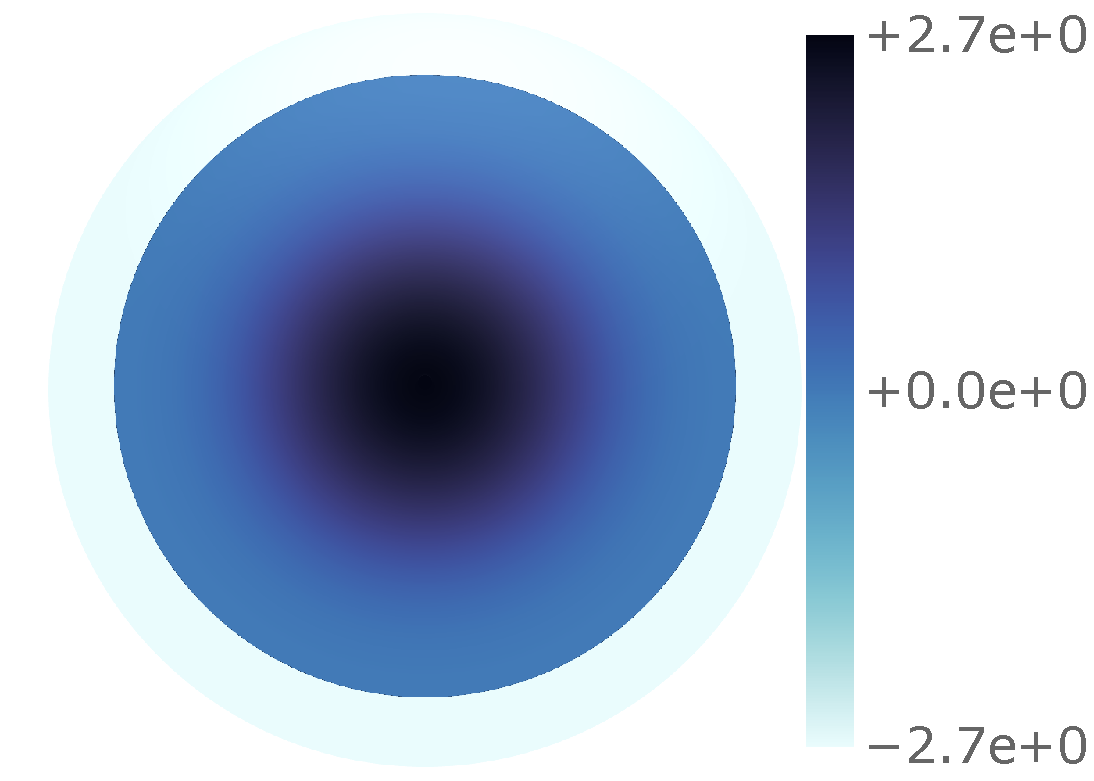
\includegraphics[trim={23 7 3 6},clip,width=.25\textwidth]{slepian_polar40_m0_rank0_lam1-000000e00_L16_res128_real.pdf}} % chktex 8
	\hfill
	\subfloat[\(\mu_{2}=0.999998\)]
	{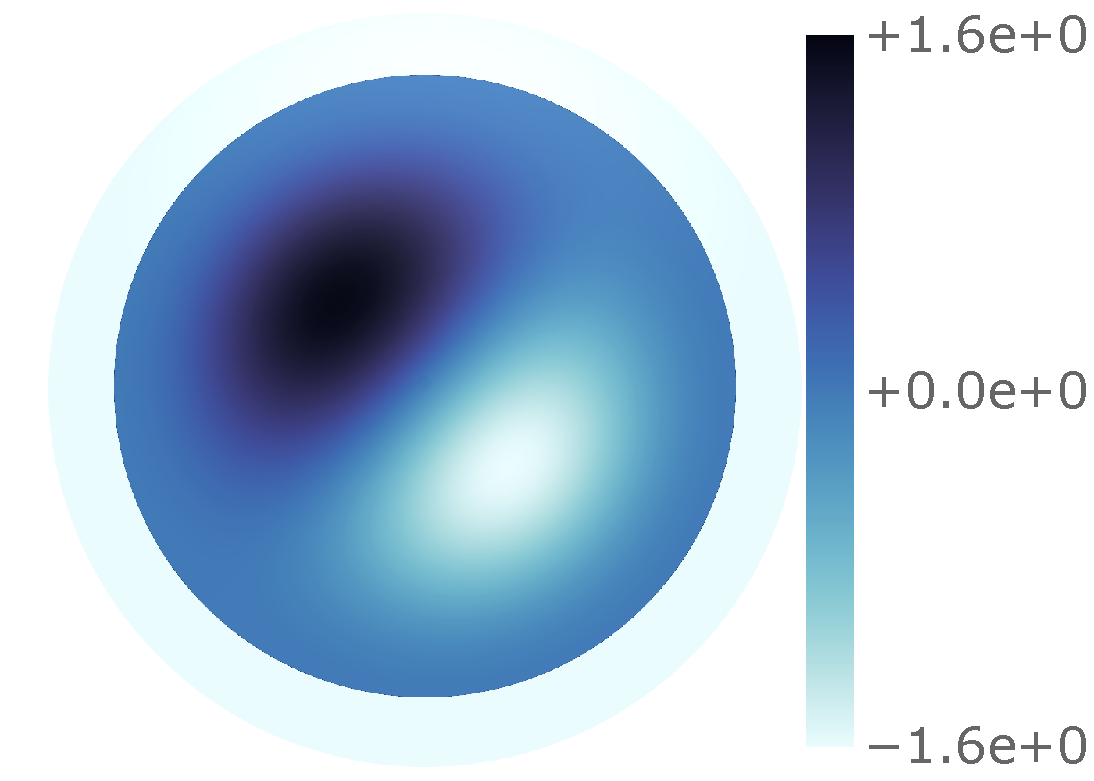
\includegraphics[trim={23 7 3 6},clip,width=.25\textwidth]{slepian_polar40_m-1_rank1_lam9-999984e-01_L16_res128_real.pdf}} % chktex 8
	\hfill
	\subfloat[\(\mu_{3}=0.999998\)]
	{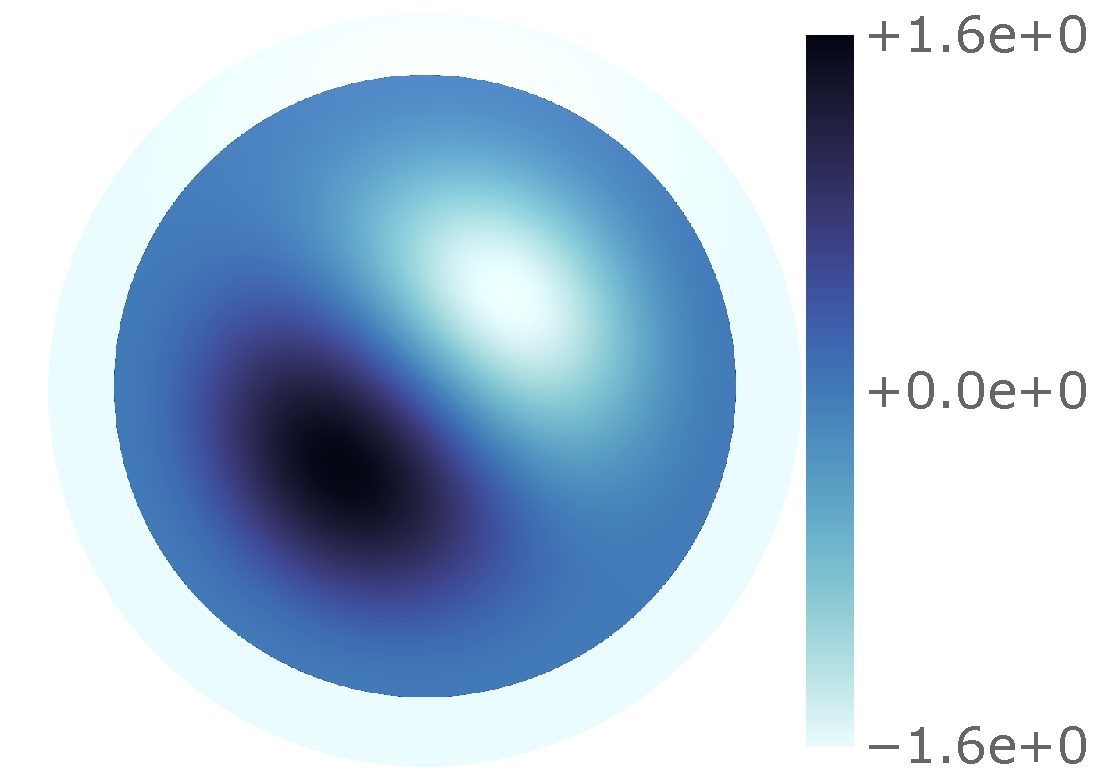
\includegraphics[trim={23 7 3 6},clip,width=.25\textwidth]{slepian_polar40_m1_rank2_lam9-999984e-01_L16_res128_real.pdf}} % chktex 8
	\hfill
	\subfloat[\(\mu_{4}=0.999966\)]
	{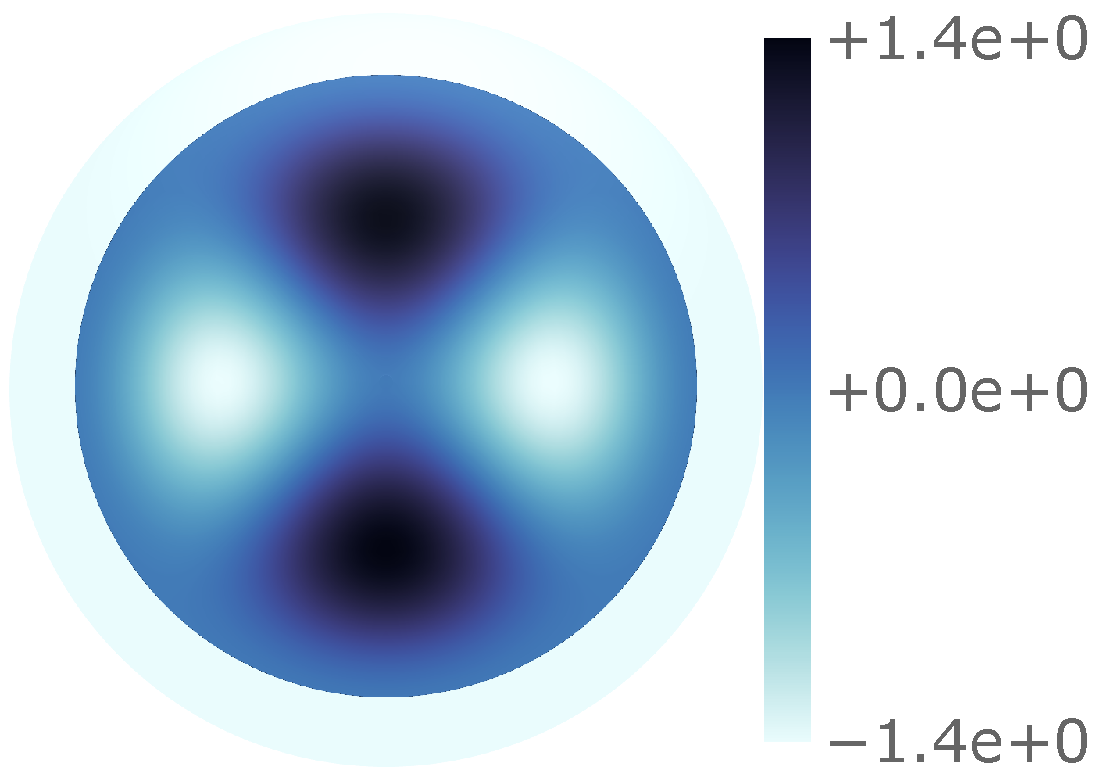
\includegraphics[trim={23 7 3 6},clip,width=.25\textwidth]{slepian_polar40_m-2_rank3_lam9-999664e-01_L16_res128_real.pdf}} % chktex 8
	\newline
	\subfloat[\(\mu_{5}=0.999966\)]
	{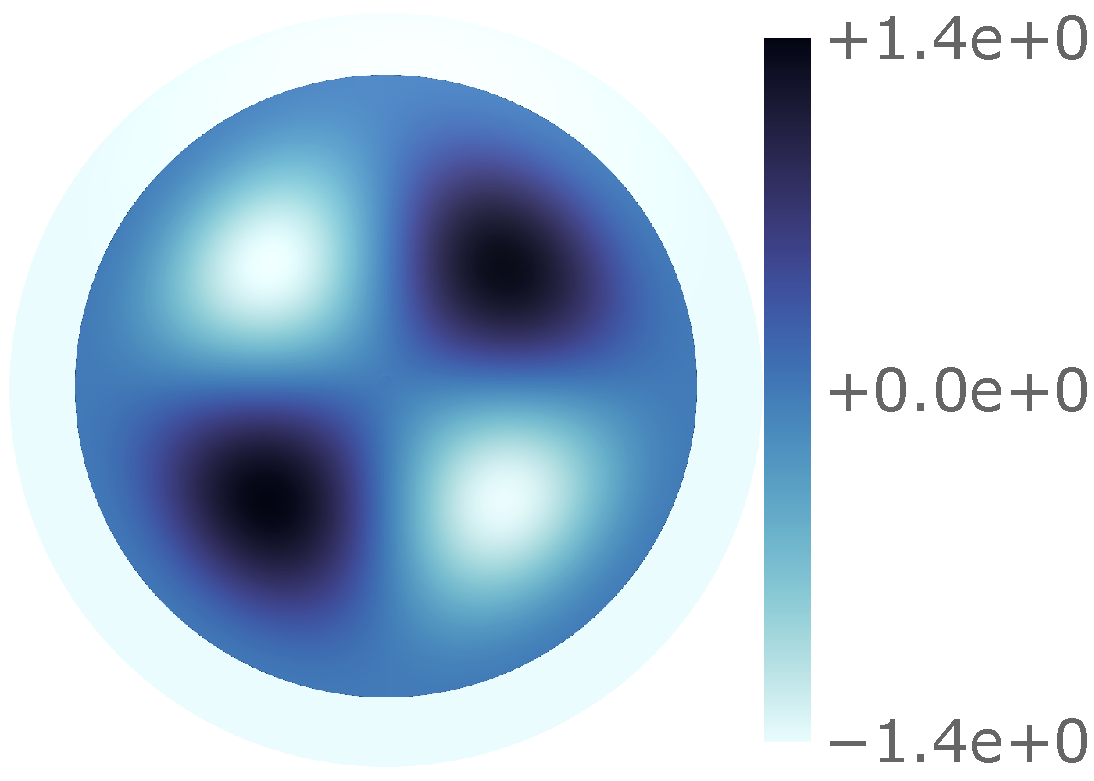
\includegraphics[trim={23 7 3 6},clip,width=.25\textwidth]{slepian_polar40_m2_rank4_lam9-999664e-01_L16_res128_real.pdf}} % chktex 8
	\hfill
	\subfloat[\(\mu_{6}=0.999939\)]
	{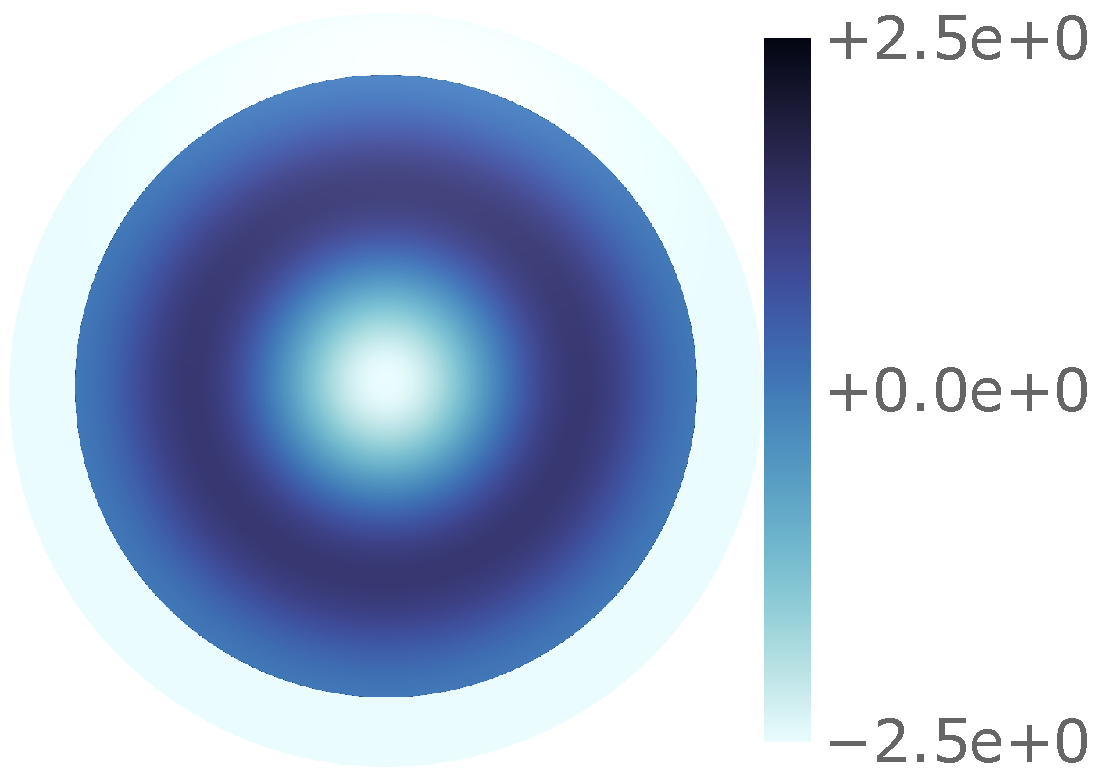
\includegraphics[trim={23 7 3 6},clip,width=.25\textwidth]{slepian_polar40_m0_rank5_lam9-999392e-01_L16_res128_real.pdf}} % chktex 8
	\hfill
	\subfloat[\(\mu_{7}=0.999553\)]
	{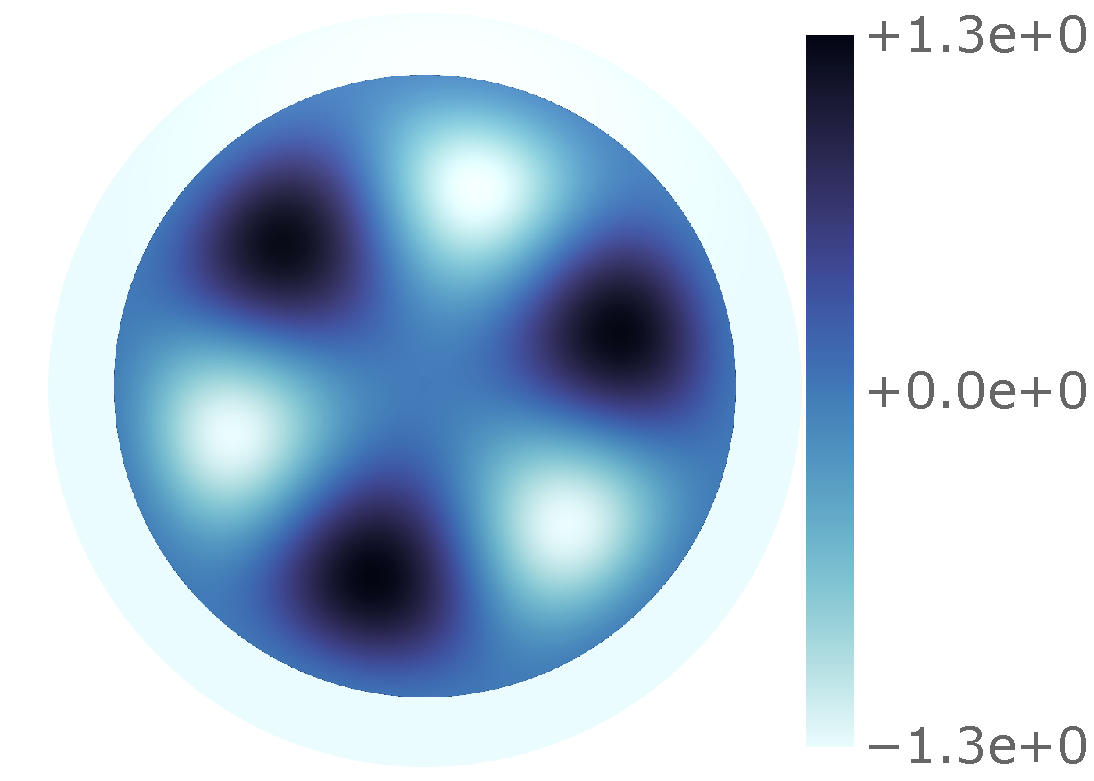
\includegraphics[trim={23 7 3 6},clip,width=.25\textwidth]{slepian_polar40_m-3_rank6_lam9-995528e-01_L16_res128_real.pdf}} % chktex 8
	\hfill
	\subfloat[\(\mu_{8}=0.999553\)]
	{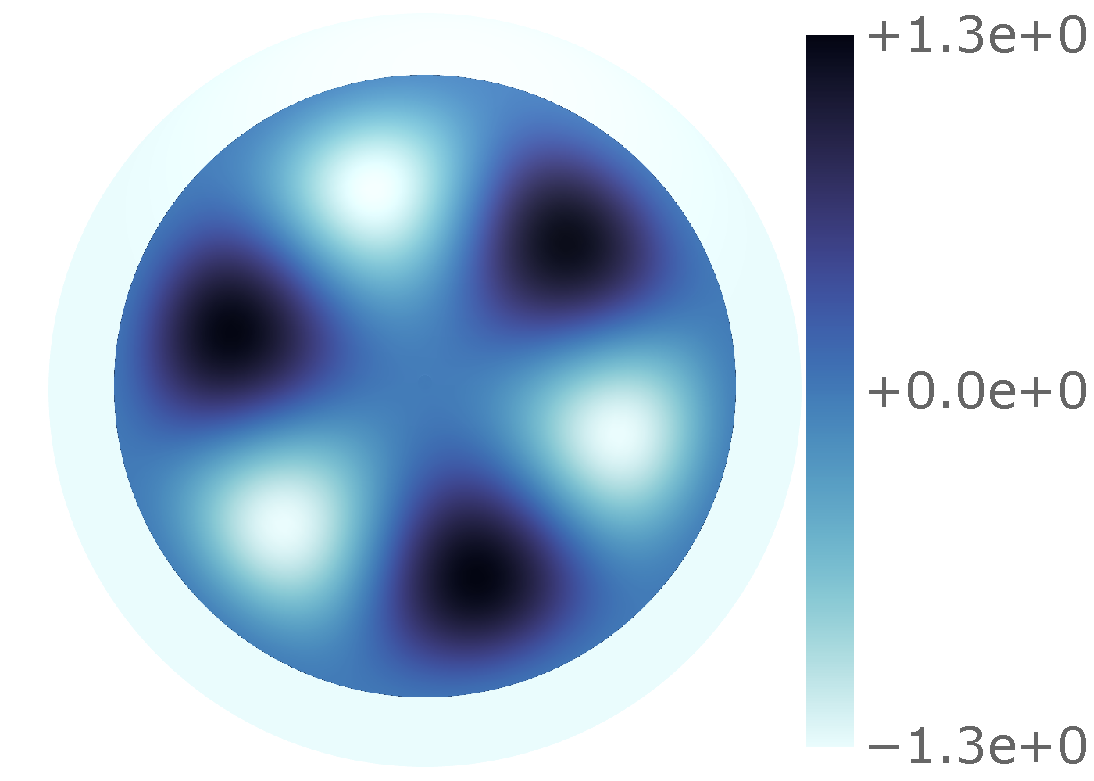
\includegraphics[trim={23 7 3 6},clip,width=.25\textwidth]{slepian_polar40_m3_rank7_lam9-995528e-01_L16_res128_real.pdf}} % chktex 8
	\newline
	\subfloat[\(\mu_{9}=0.998918\)]
	{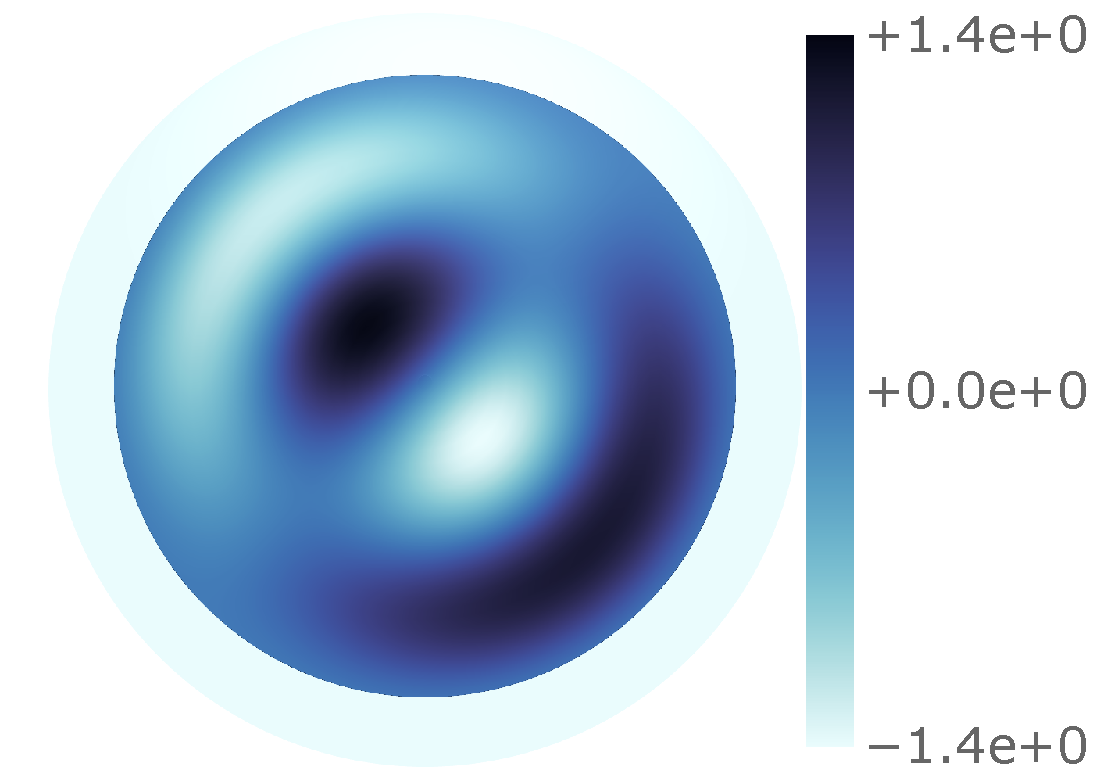
\includegraphics[trim={23 7 3 6},clip,width=.25\textwidth]{slepian_polar40_m-1_rank8_lam9-989180e-01_L16_res128_real.pdf}} % chktex 8
	\hfill
	\subfloat[\(\mu_{10}=0.998918\)]
	{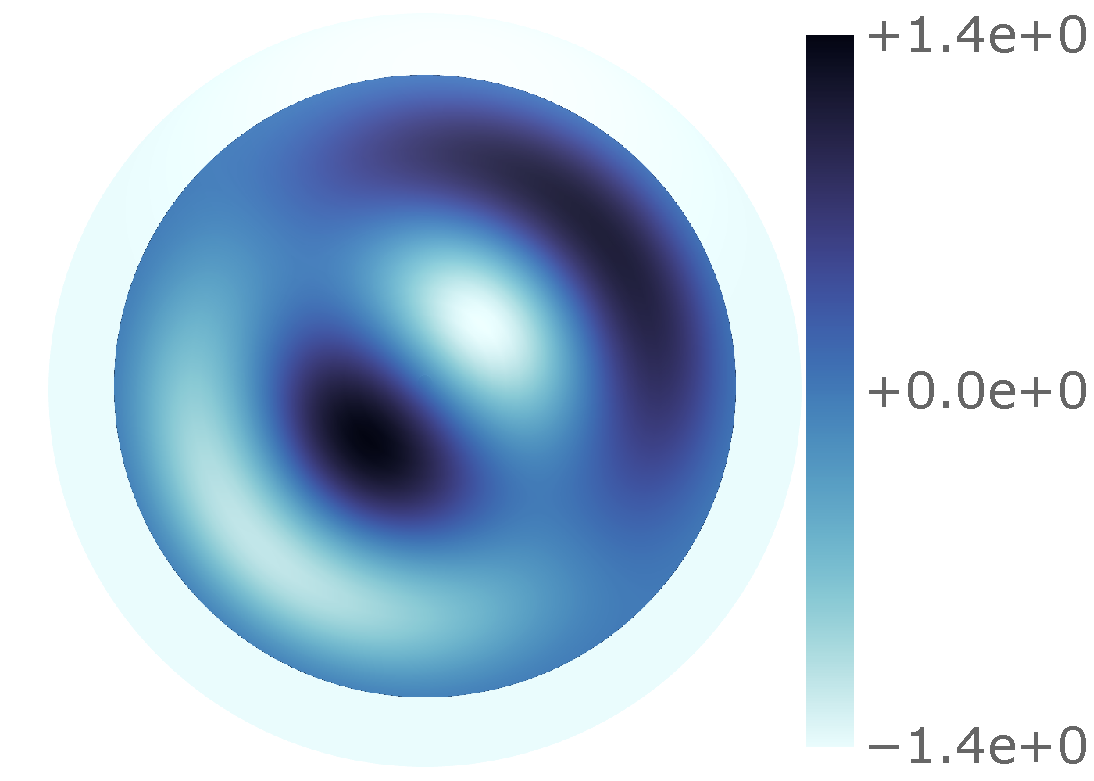
\includegraphics[trim={23 7 3 6},clip,width=.25\textwidth]{slepian_polar40_m1_rank9_lam9-989180e-01_L16_res128_real.pdf}} % chktex 8
	\hfill
	\subfloat[\(\mu_{11}=0.995897\)]
	{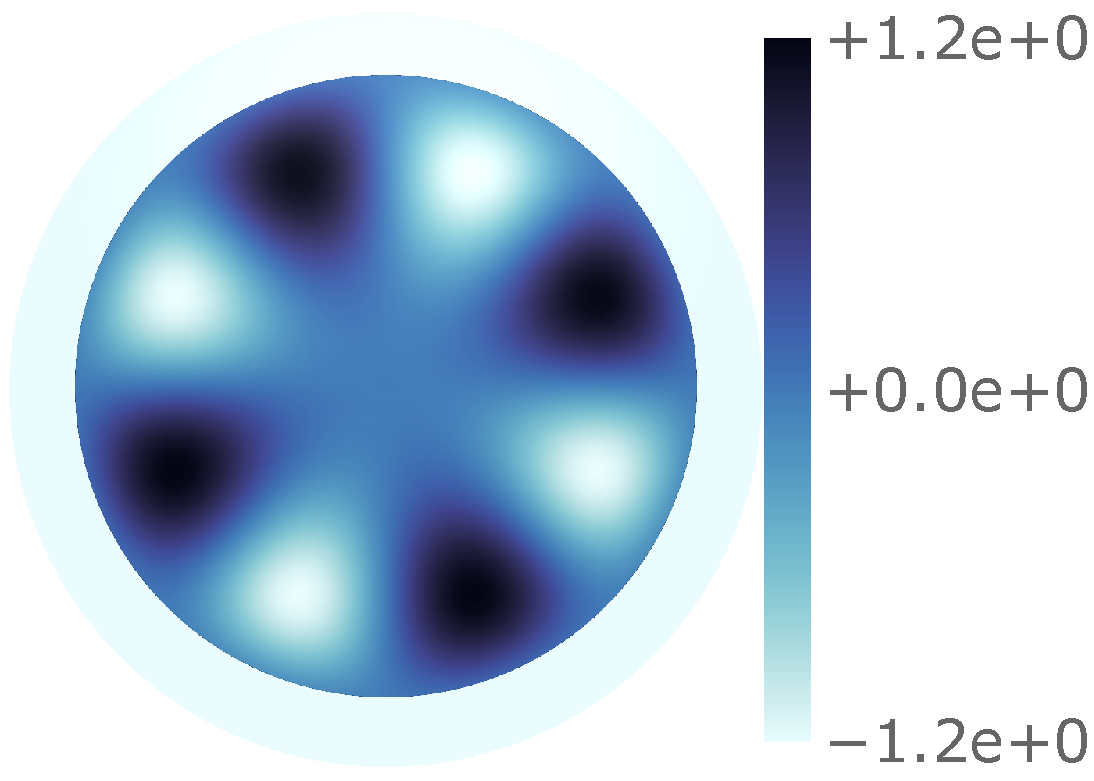
\includegraphics[trim={23 7 3 6},clip,width=.25\textwidth]{slepian_polar40_m-4_rank10_lam9-958971e-01_L16_res128_real.pdf}} % chktex 8
	\hfill
	\subfloat[\(\mu_{12}=0.995897\)]
	{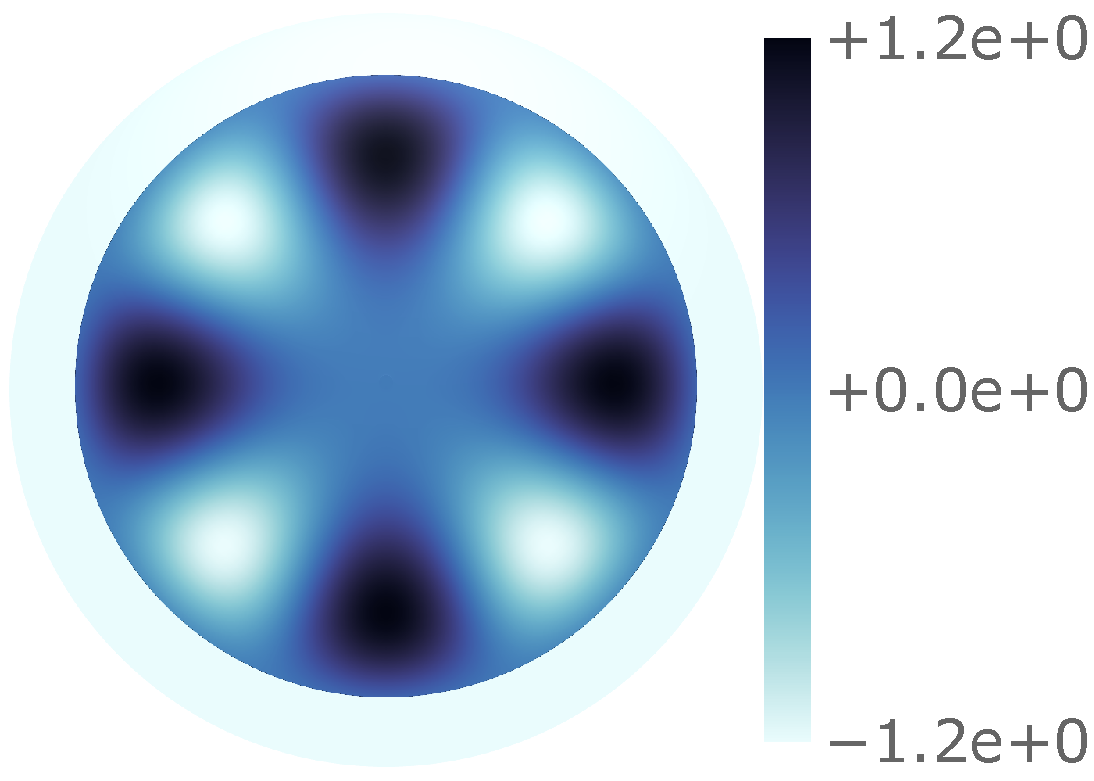
\includegraphics[trim={23 7 3 6},clip,width=.25\textwidth]{slepian_polar40_m4_rank11_lam9-958971e-01_L16_res128_real.pdf}} % chktex 8
	\newline
	\subfloat[\(\mu_{13}=0.988469\)]
	{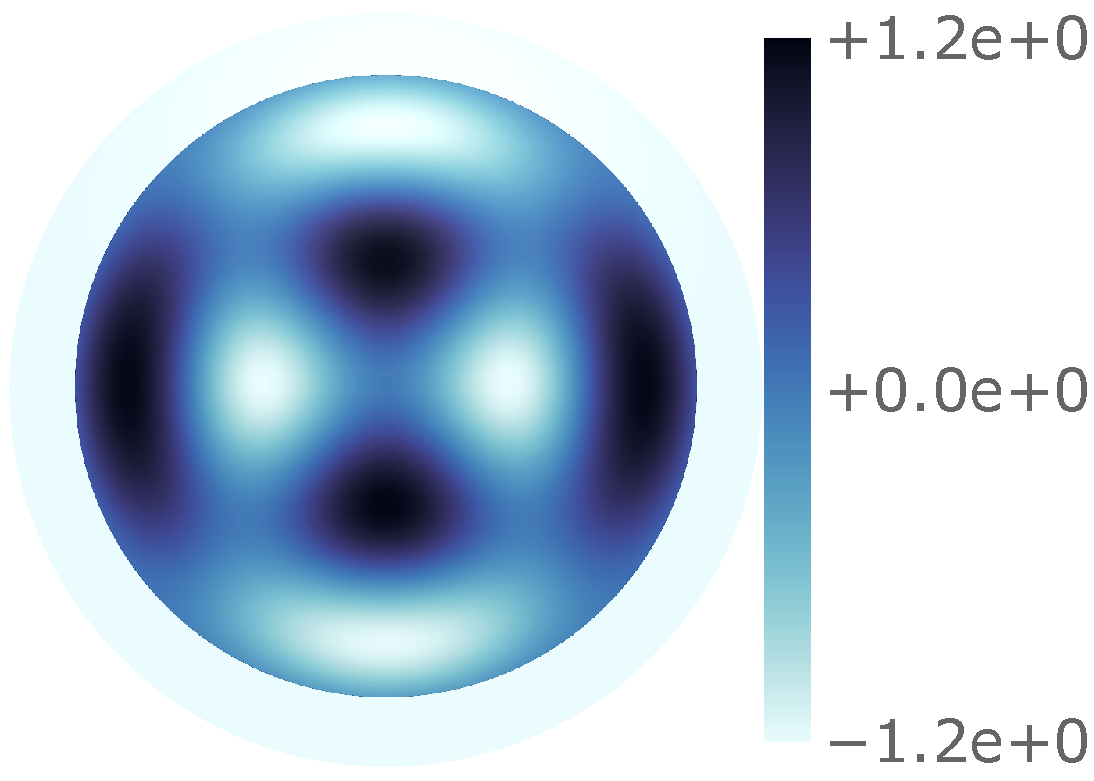
\includegraphics[trim={23 7 3 6},clip,width=.25\textwidth]{slepian_polar40_m-2_rank13_lam9-884688e-01_L16_res128_real.pdf}} % chktex 8
	\hfill
	\subfloat[\(\mu_{14}=0.988469\)]
	{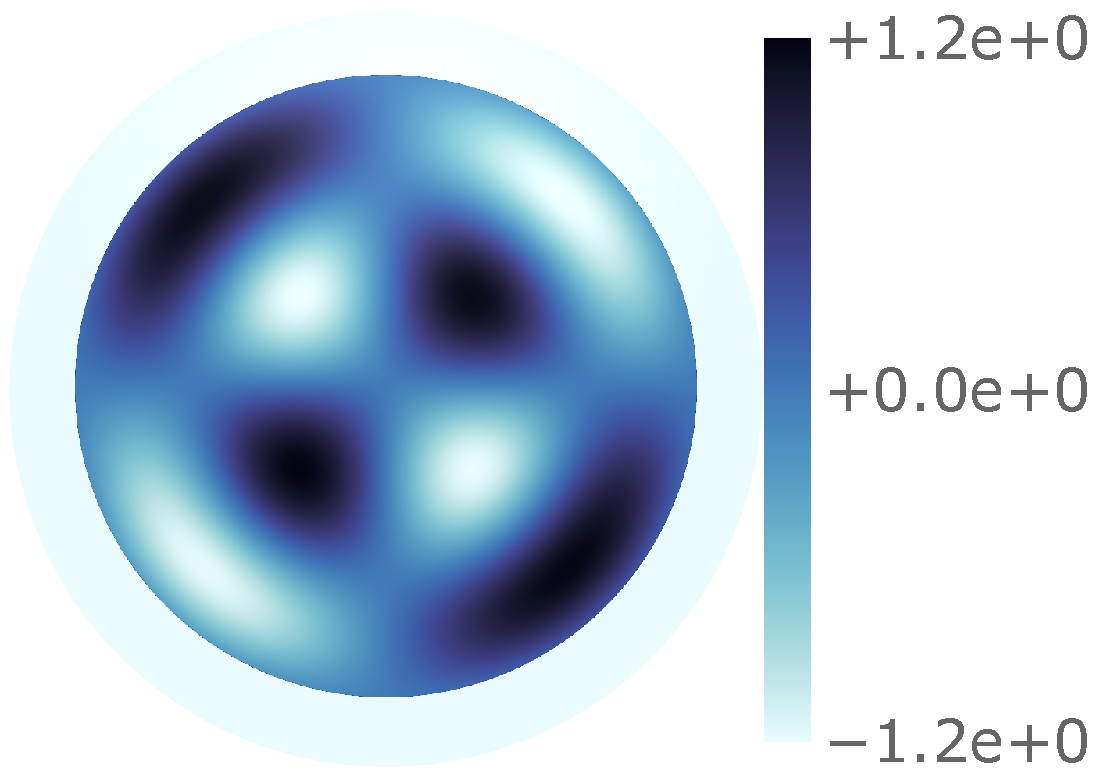
\includegraphics[trim={23 7 3 6},clip,width=.25\textwidth]{slepian_polar40_m2_rank12_lam9-884688e-01_L16_res128_real.pdf}} % chktex 8
	\hfill
	\subfloat[\(\mu_{15}=0.984654\)]
	{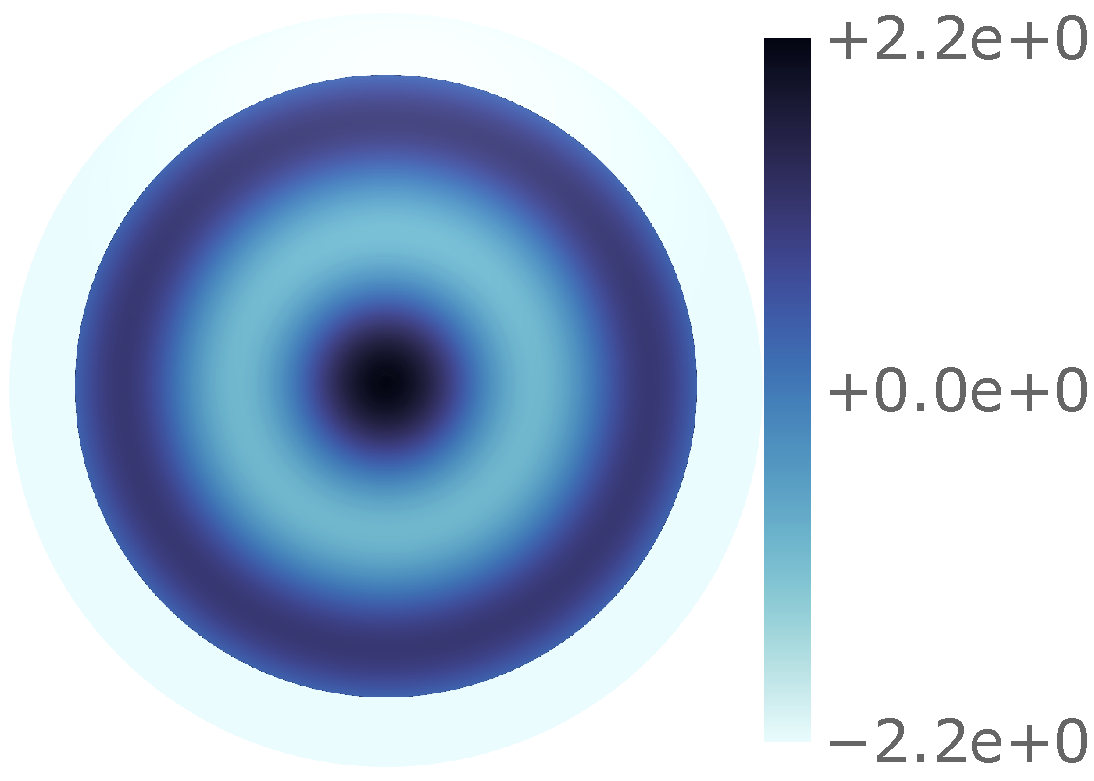
\includegraphics[trim={23 7 3 6},clip,width=.25\textwidth]{slepian_polar40_m0_rank14_lam9-846542e-01_L16_res128_real.pdf}} % chktex 8
	\hfill
	\subfloat[\(\mu_{16}=0.973439\)]
	{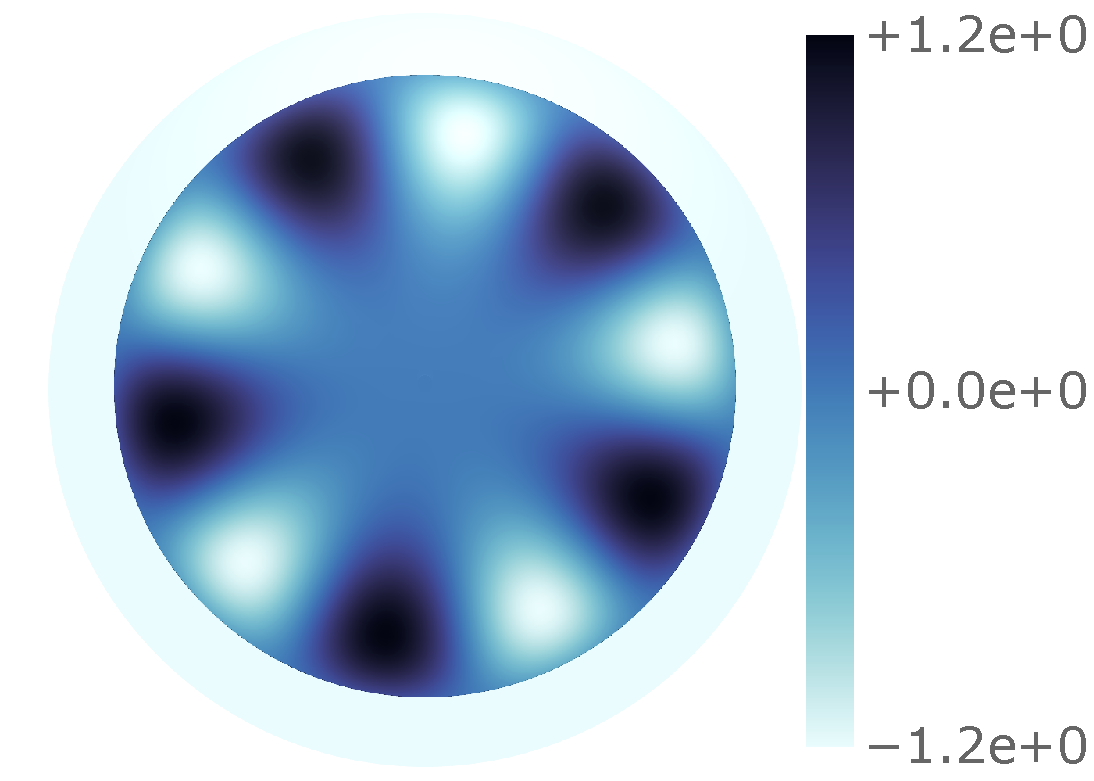
\includegraphics[trim={23 7 3 6},clip,width=.25\textwidth]{slepian_polar40_m5_rank15_lam9-734390e-01_L16_res128_real.pdf}} % chktex 8
	\caption[
		The Slepian functions within a \(\SI{40}{\degree}\) polar cap
	]{
		The first sixteen Slepian functions \(\pixel{\slepian{S}}\) within a polar cap of colatitudinal radius \(\Theta_{0}=\SI{40}{\degree}\).
		The bandlimit here is  \(L=16\), which corresponds to a Shannon number of \(N=30\).
		Ordered by decreasing eigenvalue, the plots are shown left-to-right, top-to-bottom --- indicating worse concentration within the region.
		Note the similarity with the spherical harmonics in this straightforward region.
	}\label{fig:chapter2_slepian_polar_cap}
\end{figure}


\begin{figure}[htpb]
	\centering\capstart{}
	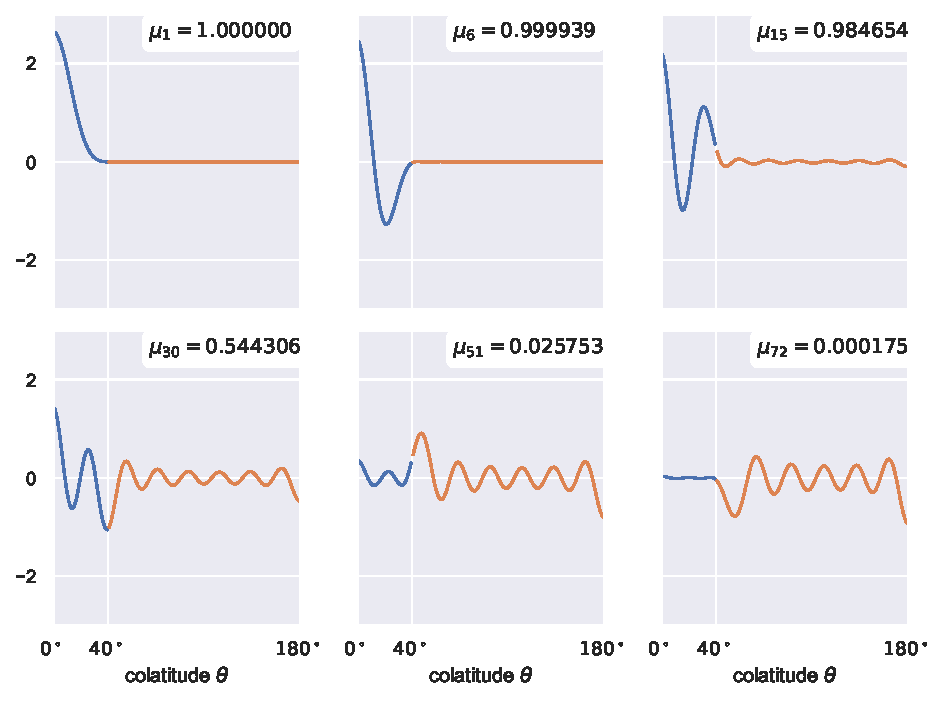
\includegraphics[width=\textwidth]{slepian_colatitude.pdf}
	\caption[
		The colatitudinal dependence of the polar cap Slepian functions
	]{
		The colatitudinal dependence of the Slepian functions \(\pixel{\slepian{S}}\) within a polar cap of colatitudinal radius \(\Theta_{0}=\SI{40}{\degree}\) for \(p \in \set{1, 6, 15, 30, 51, 72}\) shown left-to-right, top-to-bottom.
		The bandlimit here is  \(L=16\), which corresponds to a Shannon number of \(N=30\), \ie{} the final two panels are beyond the Shannon number.
		Blue curves show the concentration within the cap \(\SI{0}{\degree} \leq \theta \leq \Theta_{0}{}\), whilst orange curves show the leakage into the rest of the sphere \(\Theta_{0} < \theta \leq \SI{180}{\degree}\).
		The eigenvalue \(\mu{}\) quantifies the relative spatial concentration of the Slepian function, where lower values have increasing leakage into the orange curve.
	}\label{fig:chapter2_slepian_colatitude}
\end{figure}


\begin{figure}[htpb]
	\centering\capstart{}
	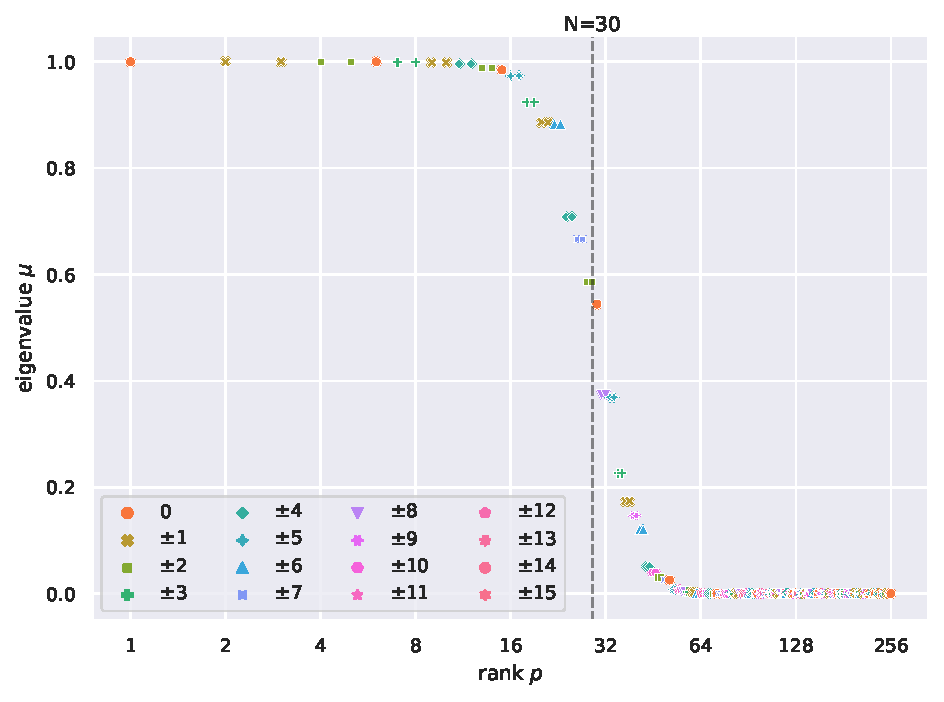
\includegraphics[width=\textwidth]{polar_cap_eigenvalues.pdf}
	\caption[
		The Slepian eigenvalues within a \(\SI{40}{\degree}\) polar cap
	]{
		The ordered Slepian eigenvalues within a polar cap of colatitudinal radius \(\theta_{0}=\SI{40}{\degree}\).
		The bandlimit here is \(L=16\), which corresponds to a Shannon number of \(N=30\), as indicated on the plot.
		Initially, the eigenvalues are \(\almost{1}\), before decreasing rapidly around the Shannon number, and where the majority of the later eigenvalues are \(\almost{0}\).
	}\label{fig:chapter2_polar_cap_eigenvalues}
\end{figure}


\section{Motivation}\label{sec:chapter2_motivation}

\subsection{Overview}

\subsection{Cosmology}

\begin{figure}[htpb]
	\centering\capstart{}
	\includegraphics[trim={0 200 0 0},clip,width=\textwidth]{planck_2018_temp_freq.pdf}
	\includegraphics[trim={1100 0 1100 2100},clip,width=\textwidth]{planck_2018_temp_freq.pdf}
	\caption[
		The 2018 \emph{Planck} maps in intensity in each frequency band
	]{
		Fluctuations of sky emission in each of nine \emph{Planck} frequency bands, after removal of a common dipole component (courtesy of \emph{The Planck Collaboration 2018}~\cite{Planck2020}).
		Note that the CMB is obstructed by the foreground microwave emissions of the Milky Way at all frequencies.
	}\label{fig:chapter2_planck_frequency}
\end{figure}


\begin{figure}[htpb]
\centering\capstart{}
\includegraphics[width=\textwidth]{planck_2018_temp_mask.pdf}
\caption[
The 2018 Planck CMB map with the \texttt{Commander} mask
]{
The Planck \texttt{Commander}~\cite{Eriksen2004,Eriksen2008,Planck2016,Planck2020a} CMB temperature map used in low-\(\ell{}\) temperature likelihood analysis, smoothed to \(\SI{60}{\arcminute}\) FWHM resolution (courtesy of The Planck Collaboration 2018~\cite{Planck2020a}).
The region in grey is the mask adopted for the likelihood analysis, which preserves \(\SI{86}{\percent}\) of the sky.
Rather than developing methods to estimate a full-sky map, Slepian wavelets offer an alternative approach in which the wavelets are constructed in the region outside the mask.
}\label{fig:chapter2_planck_masked}
\end{figure}


\subsection{Statistics of Random Fields on the Sphere}

\subsection{Observations Over the Partial Sphere}

\section{Outlook}\label{sec:chapter2_outlook}

\subsection{Current Approaches}

\subsection{This Thesis}
